\section{Appendix}
\subsection{Figures} % (fold)
\label{sec:Figures}

\begin{figure}[H]
    \centering
    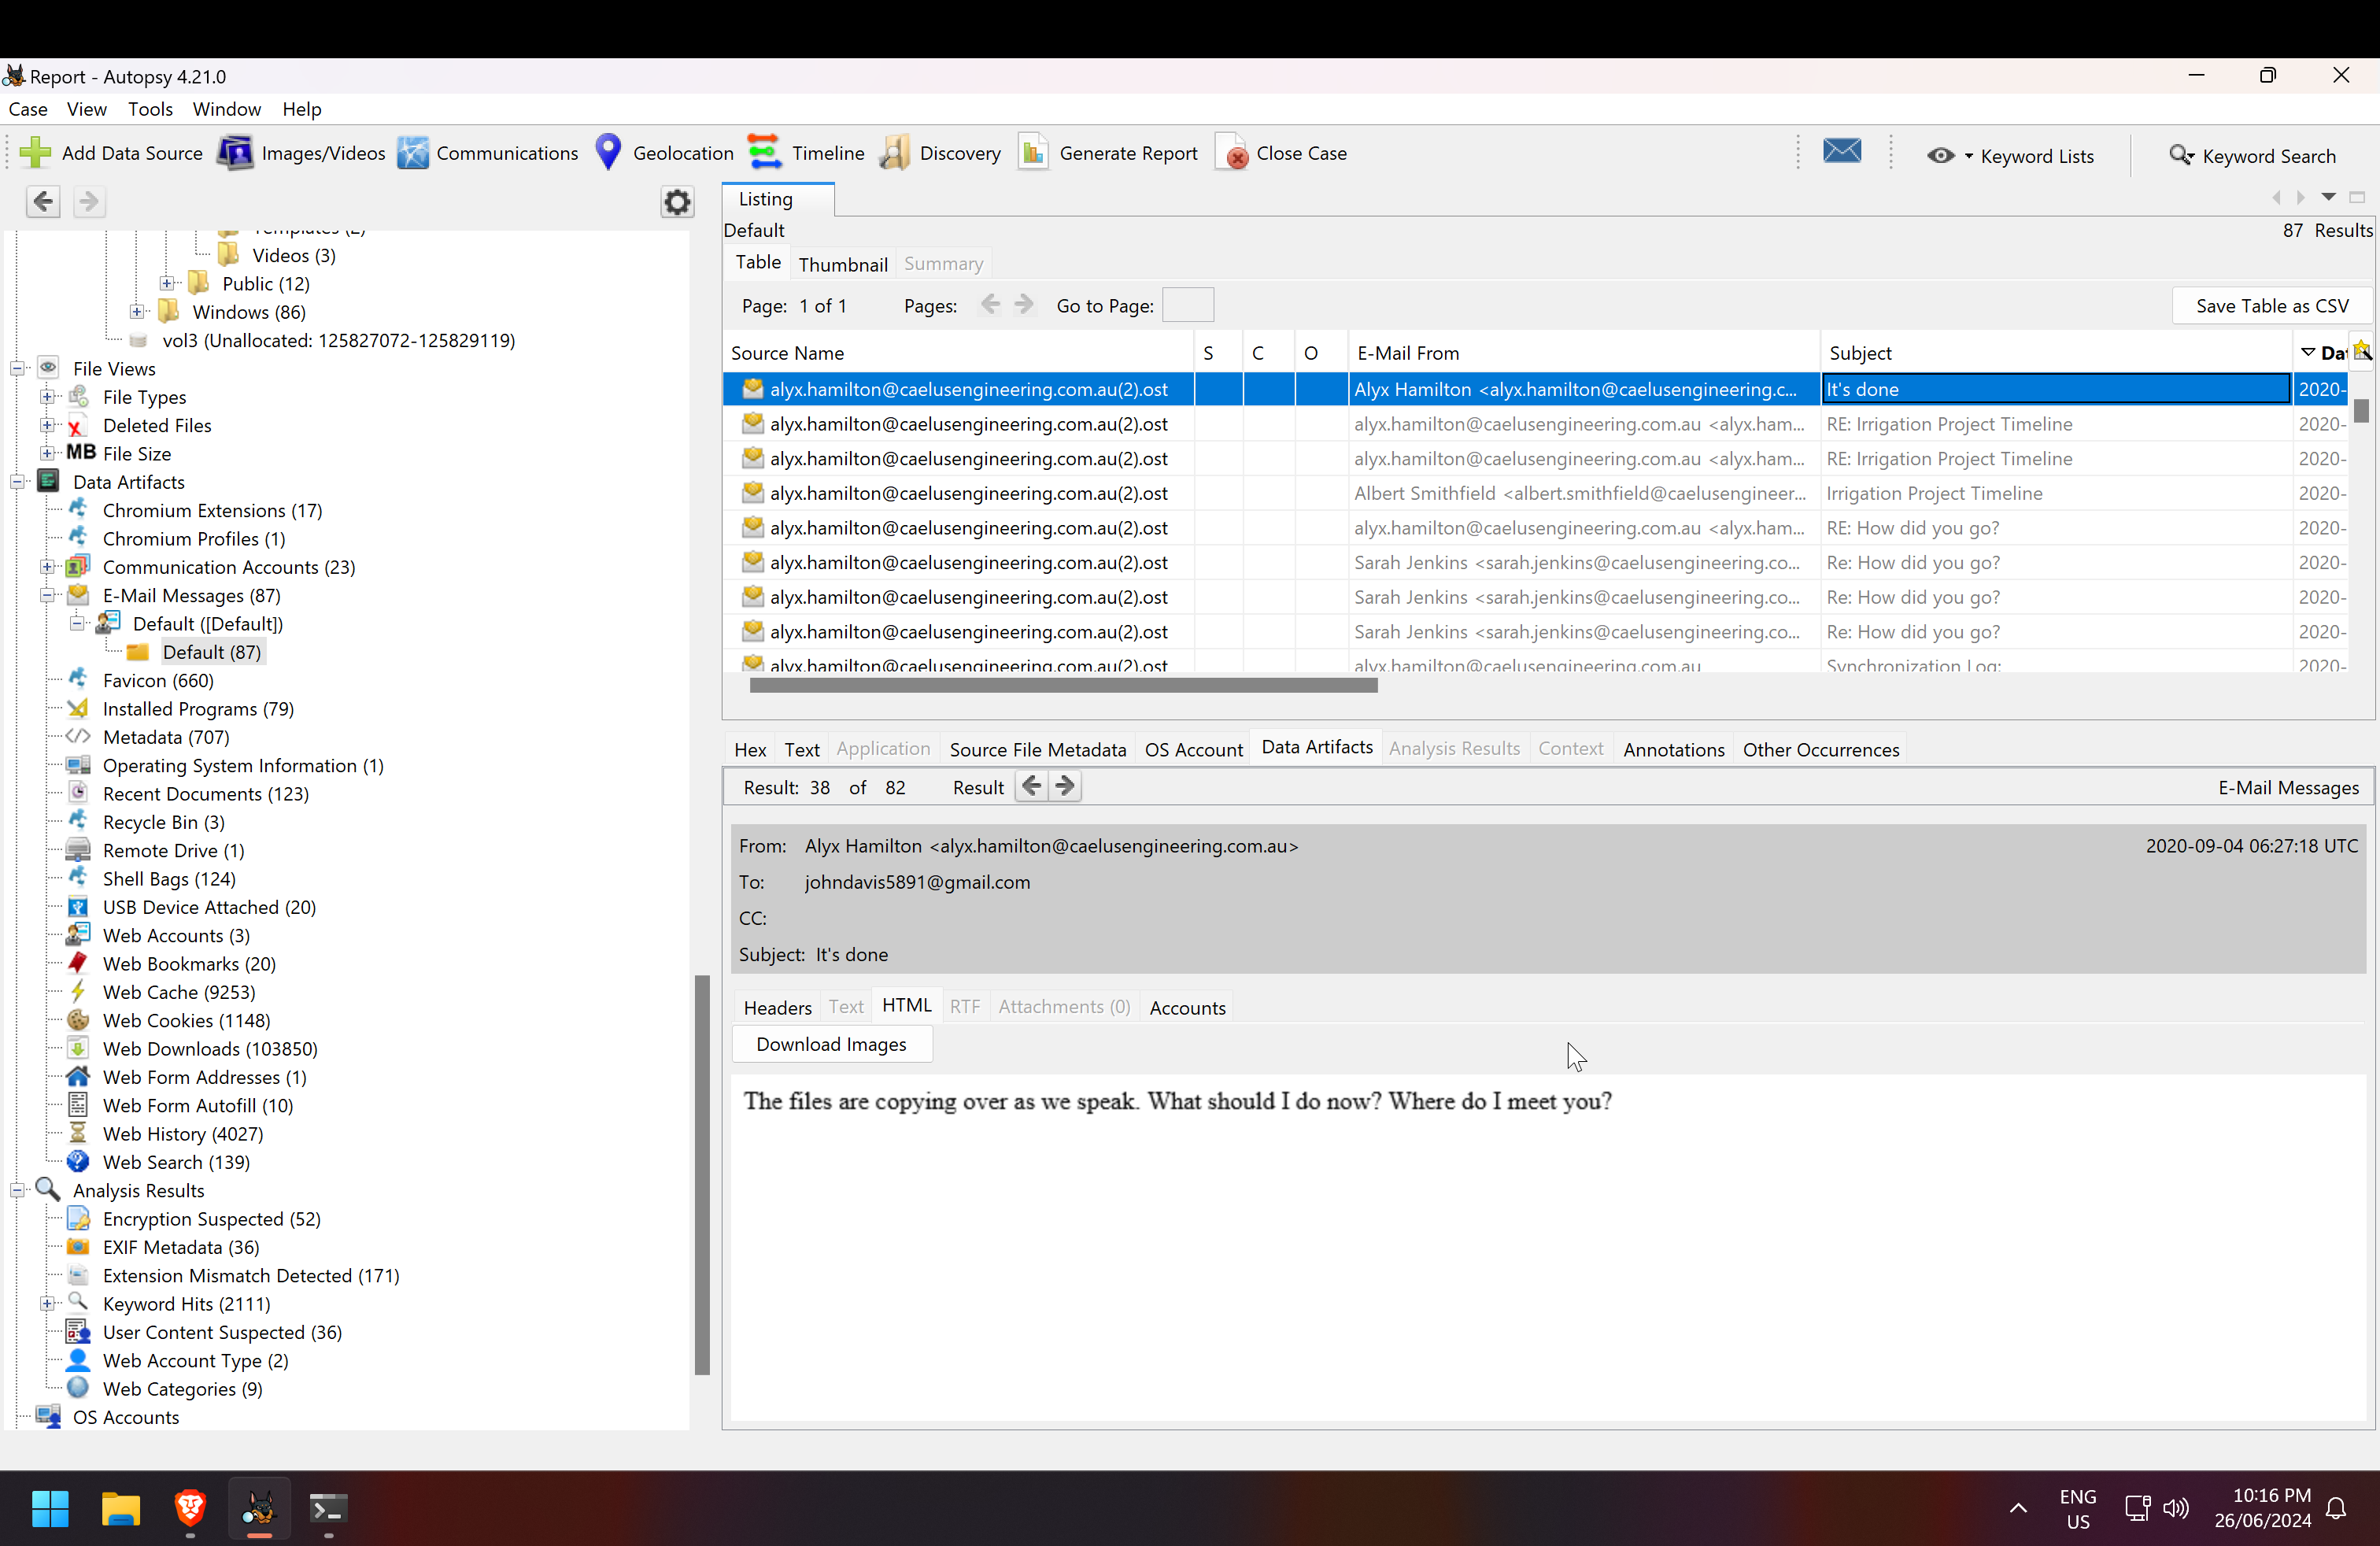
\includegraphics[width=1.0\textwidth]{email.png}
    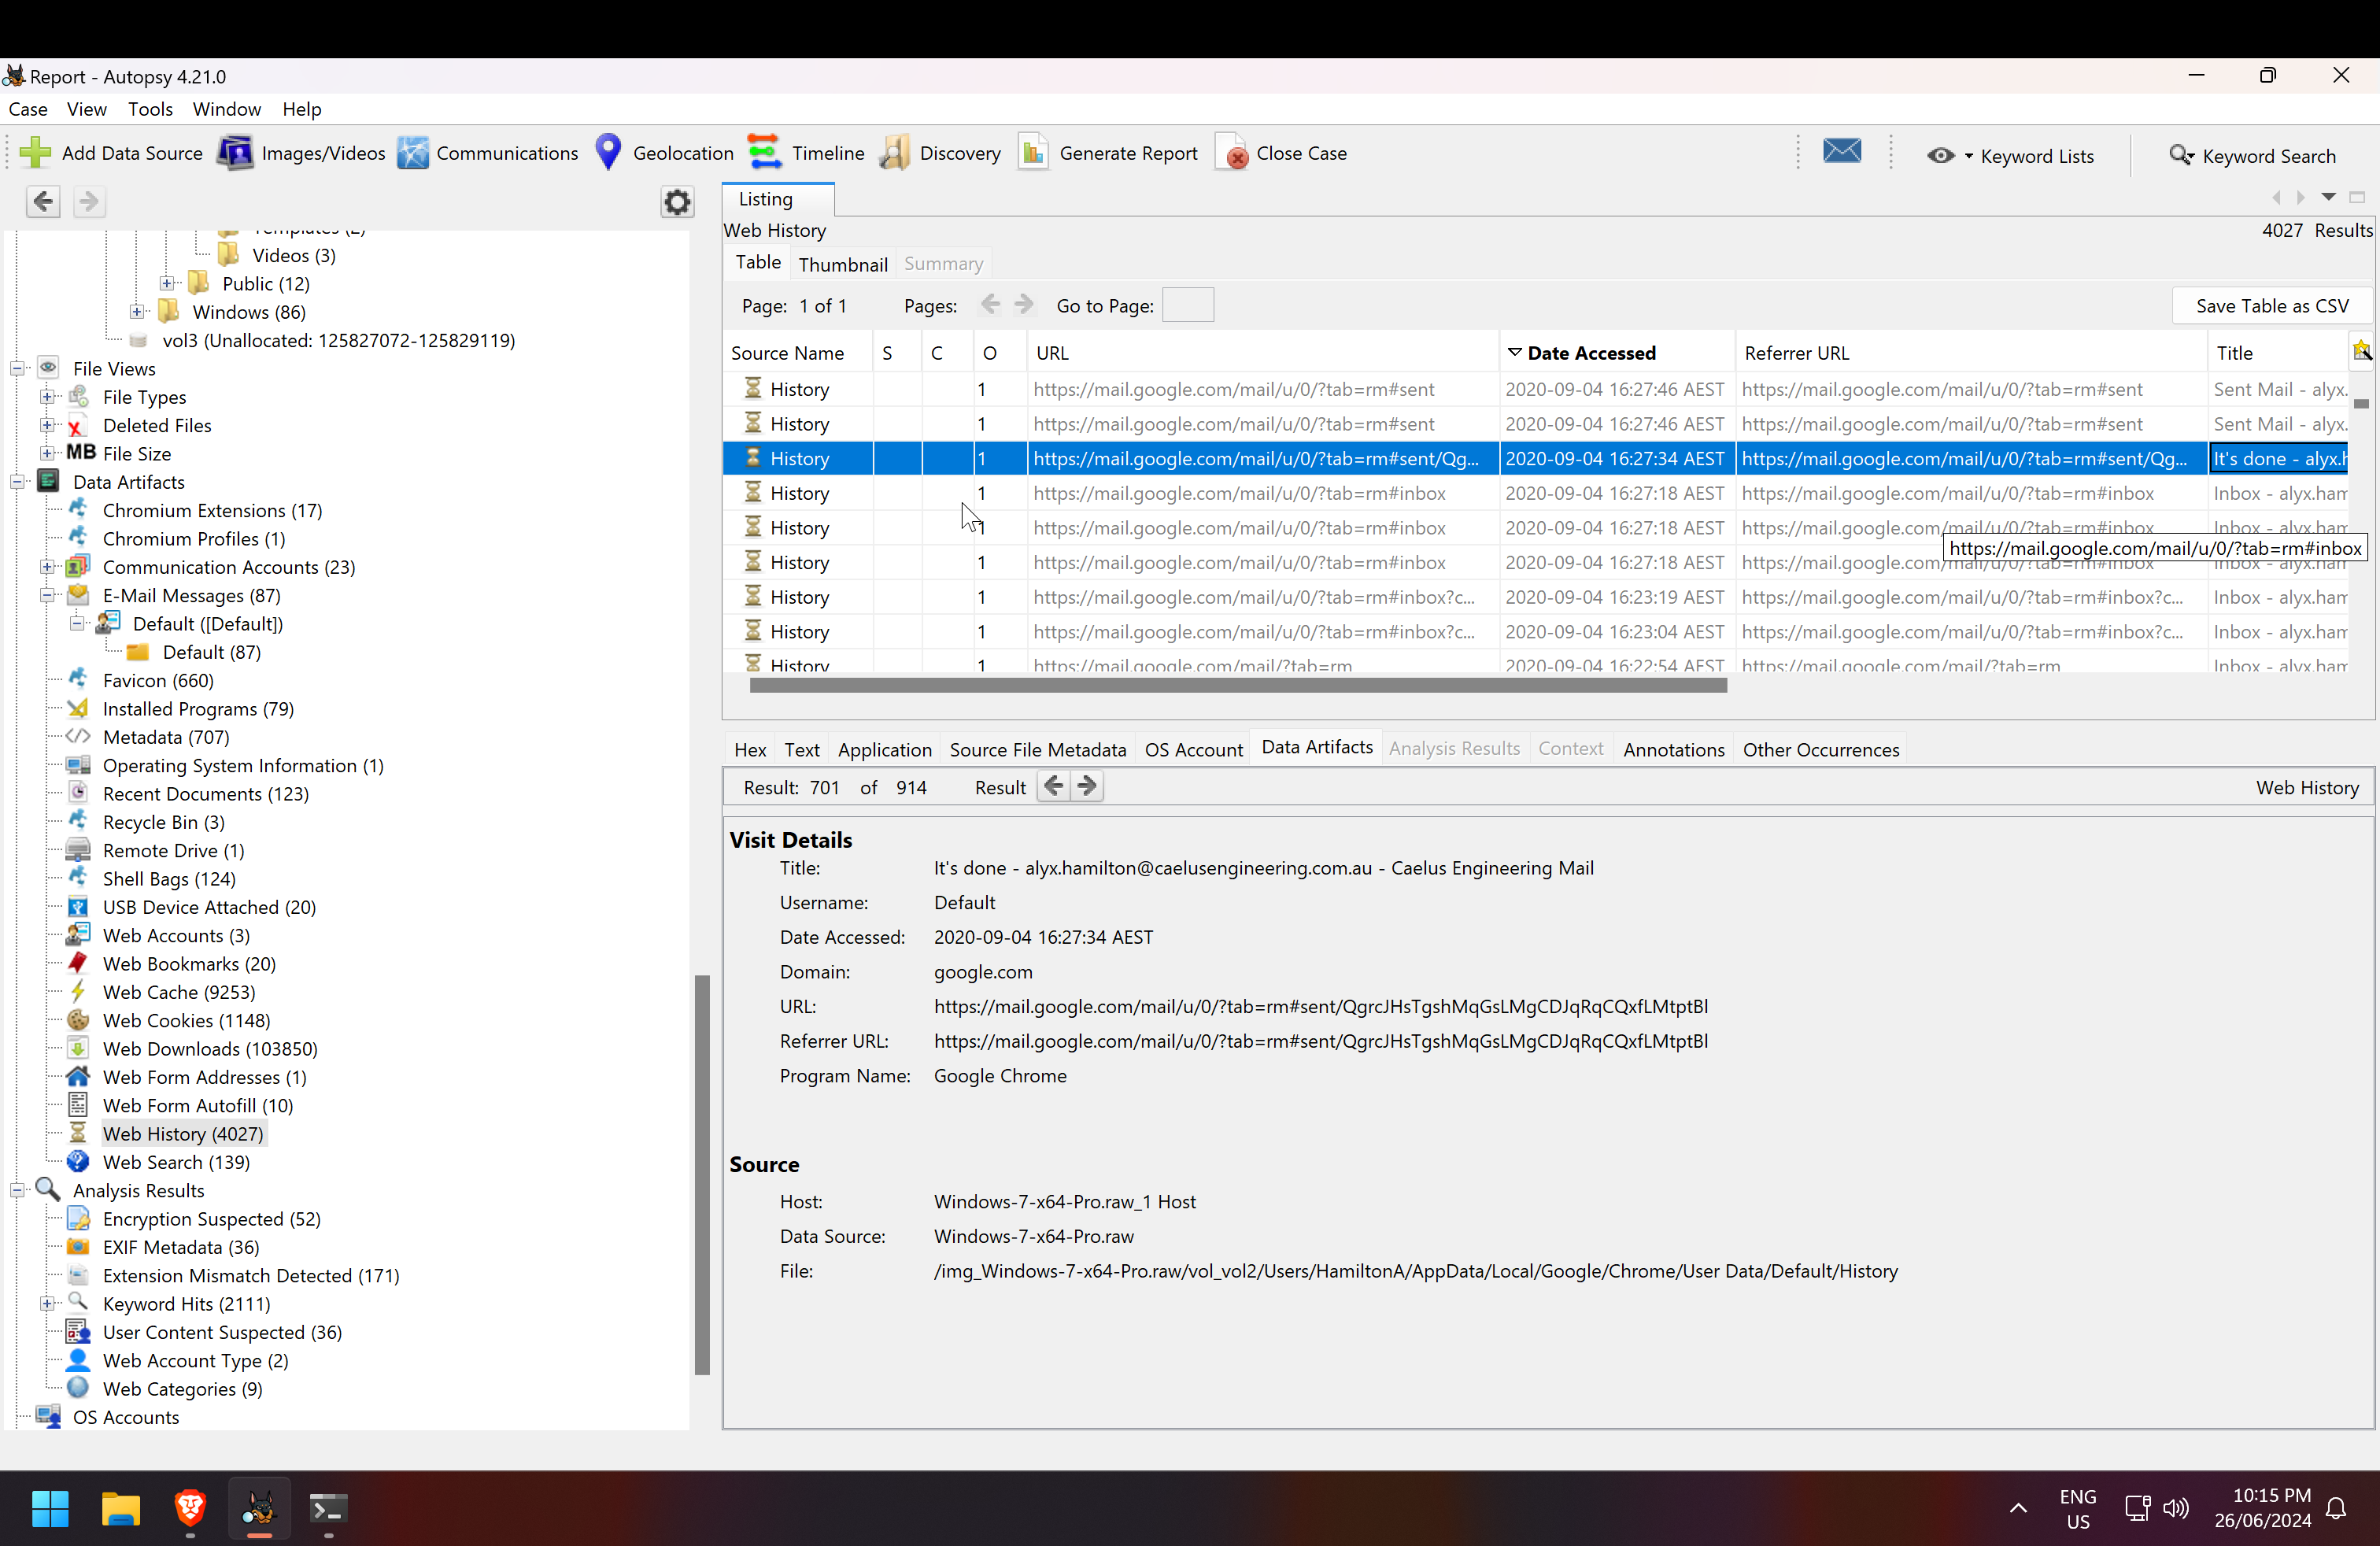
\includegraphics[width=1.0\textwidth]{email_browse_history.png}
    \caption{Cryptic email}
    \label{fig:email}
\end{figure}

\begin{figure}[H]
    \centering
    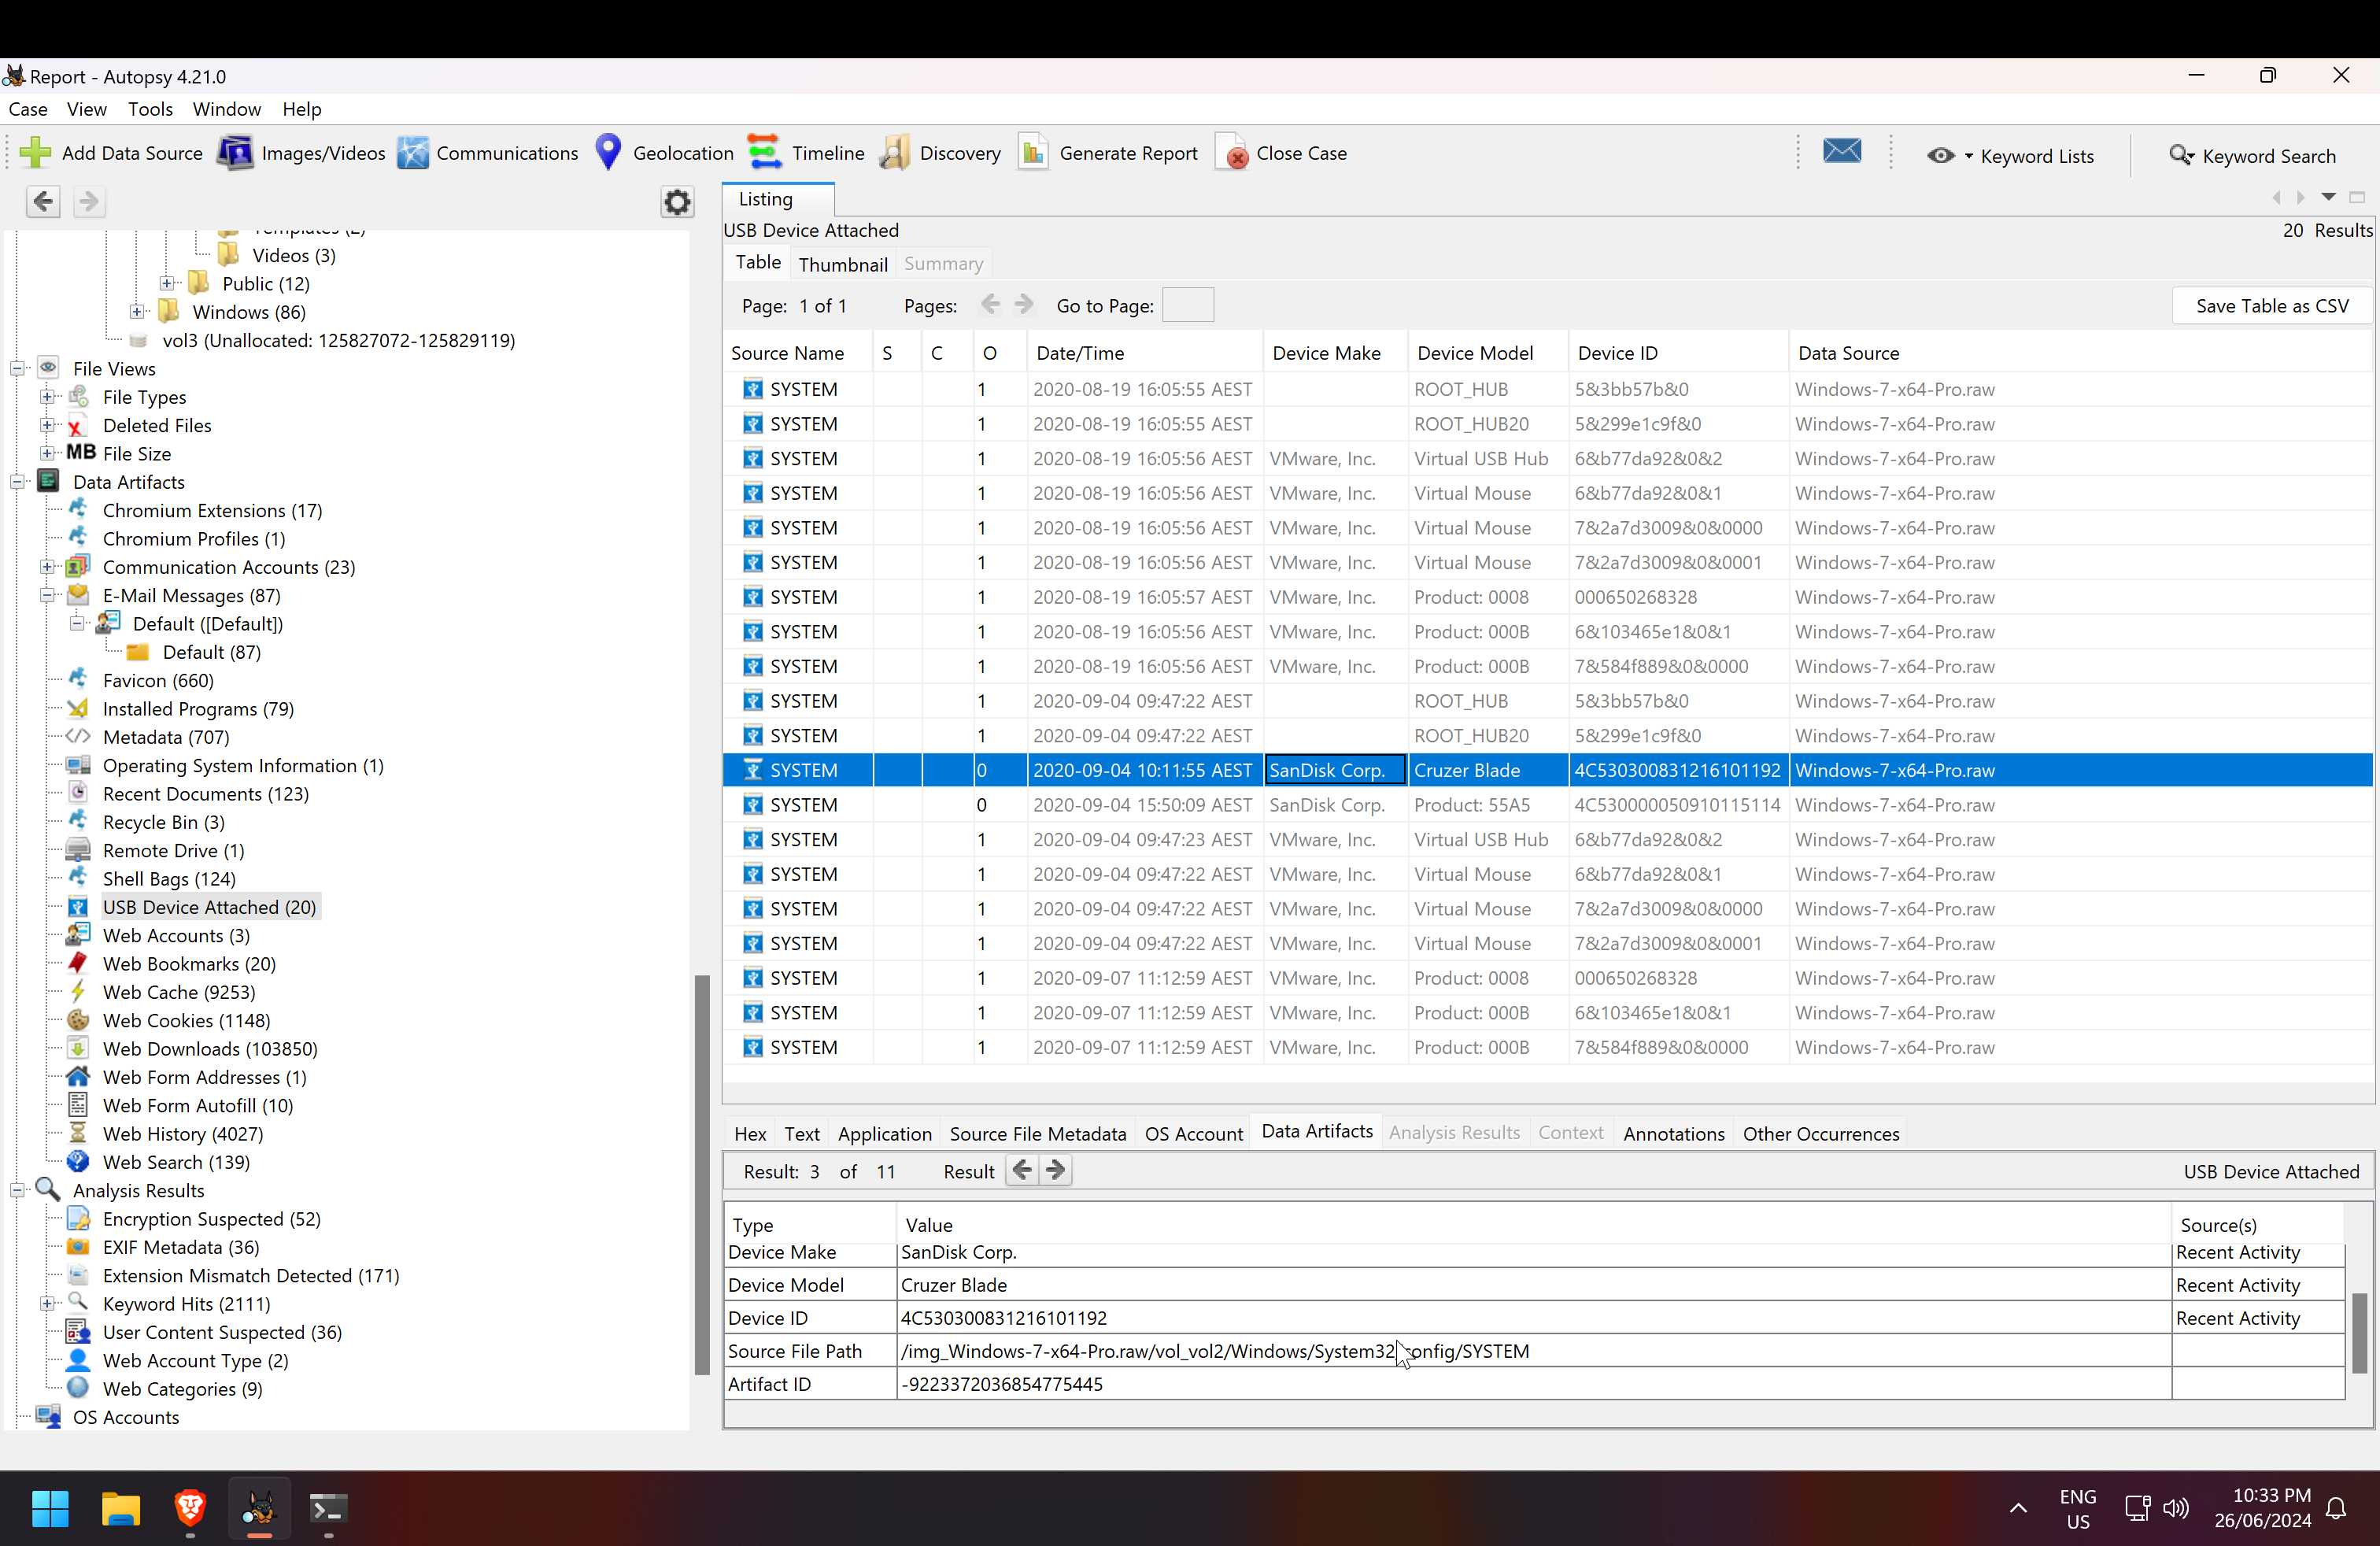
\includegraphics[width=1.0\textwidth]{usb1.png}
    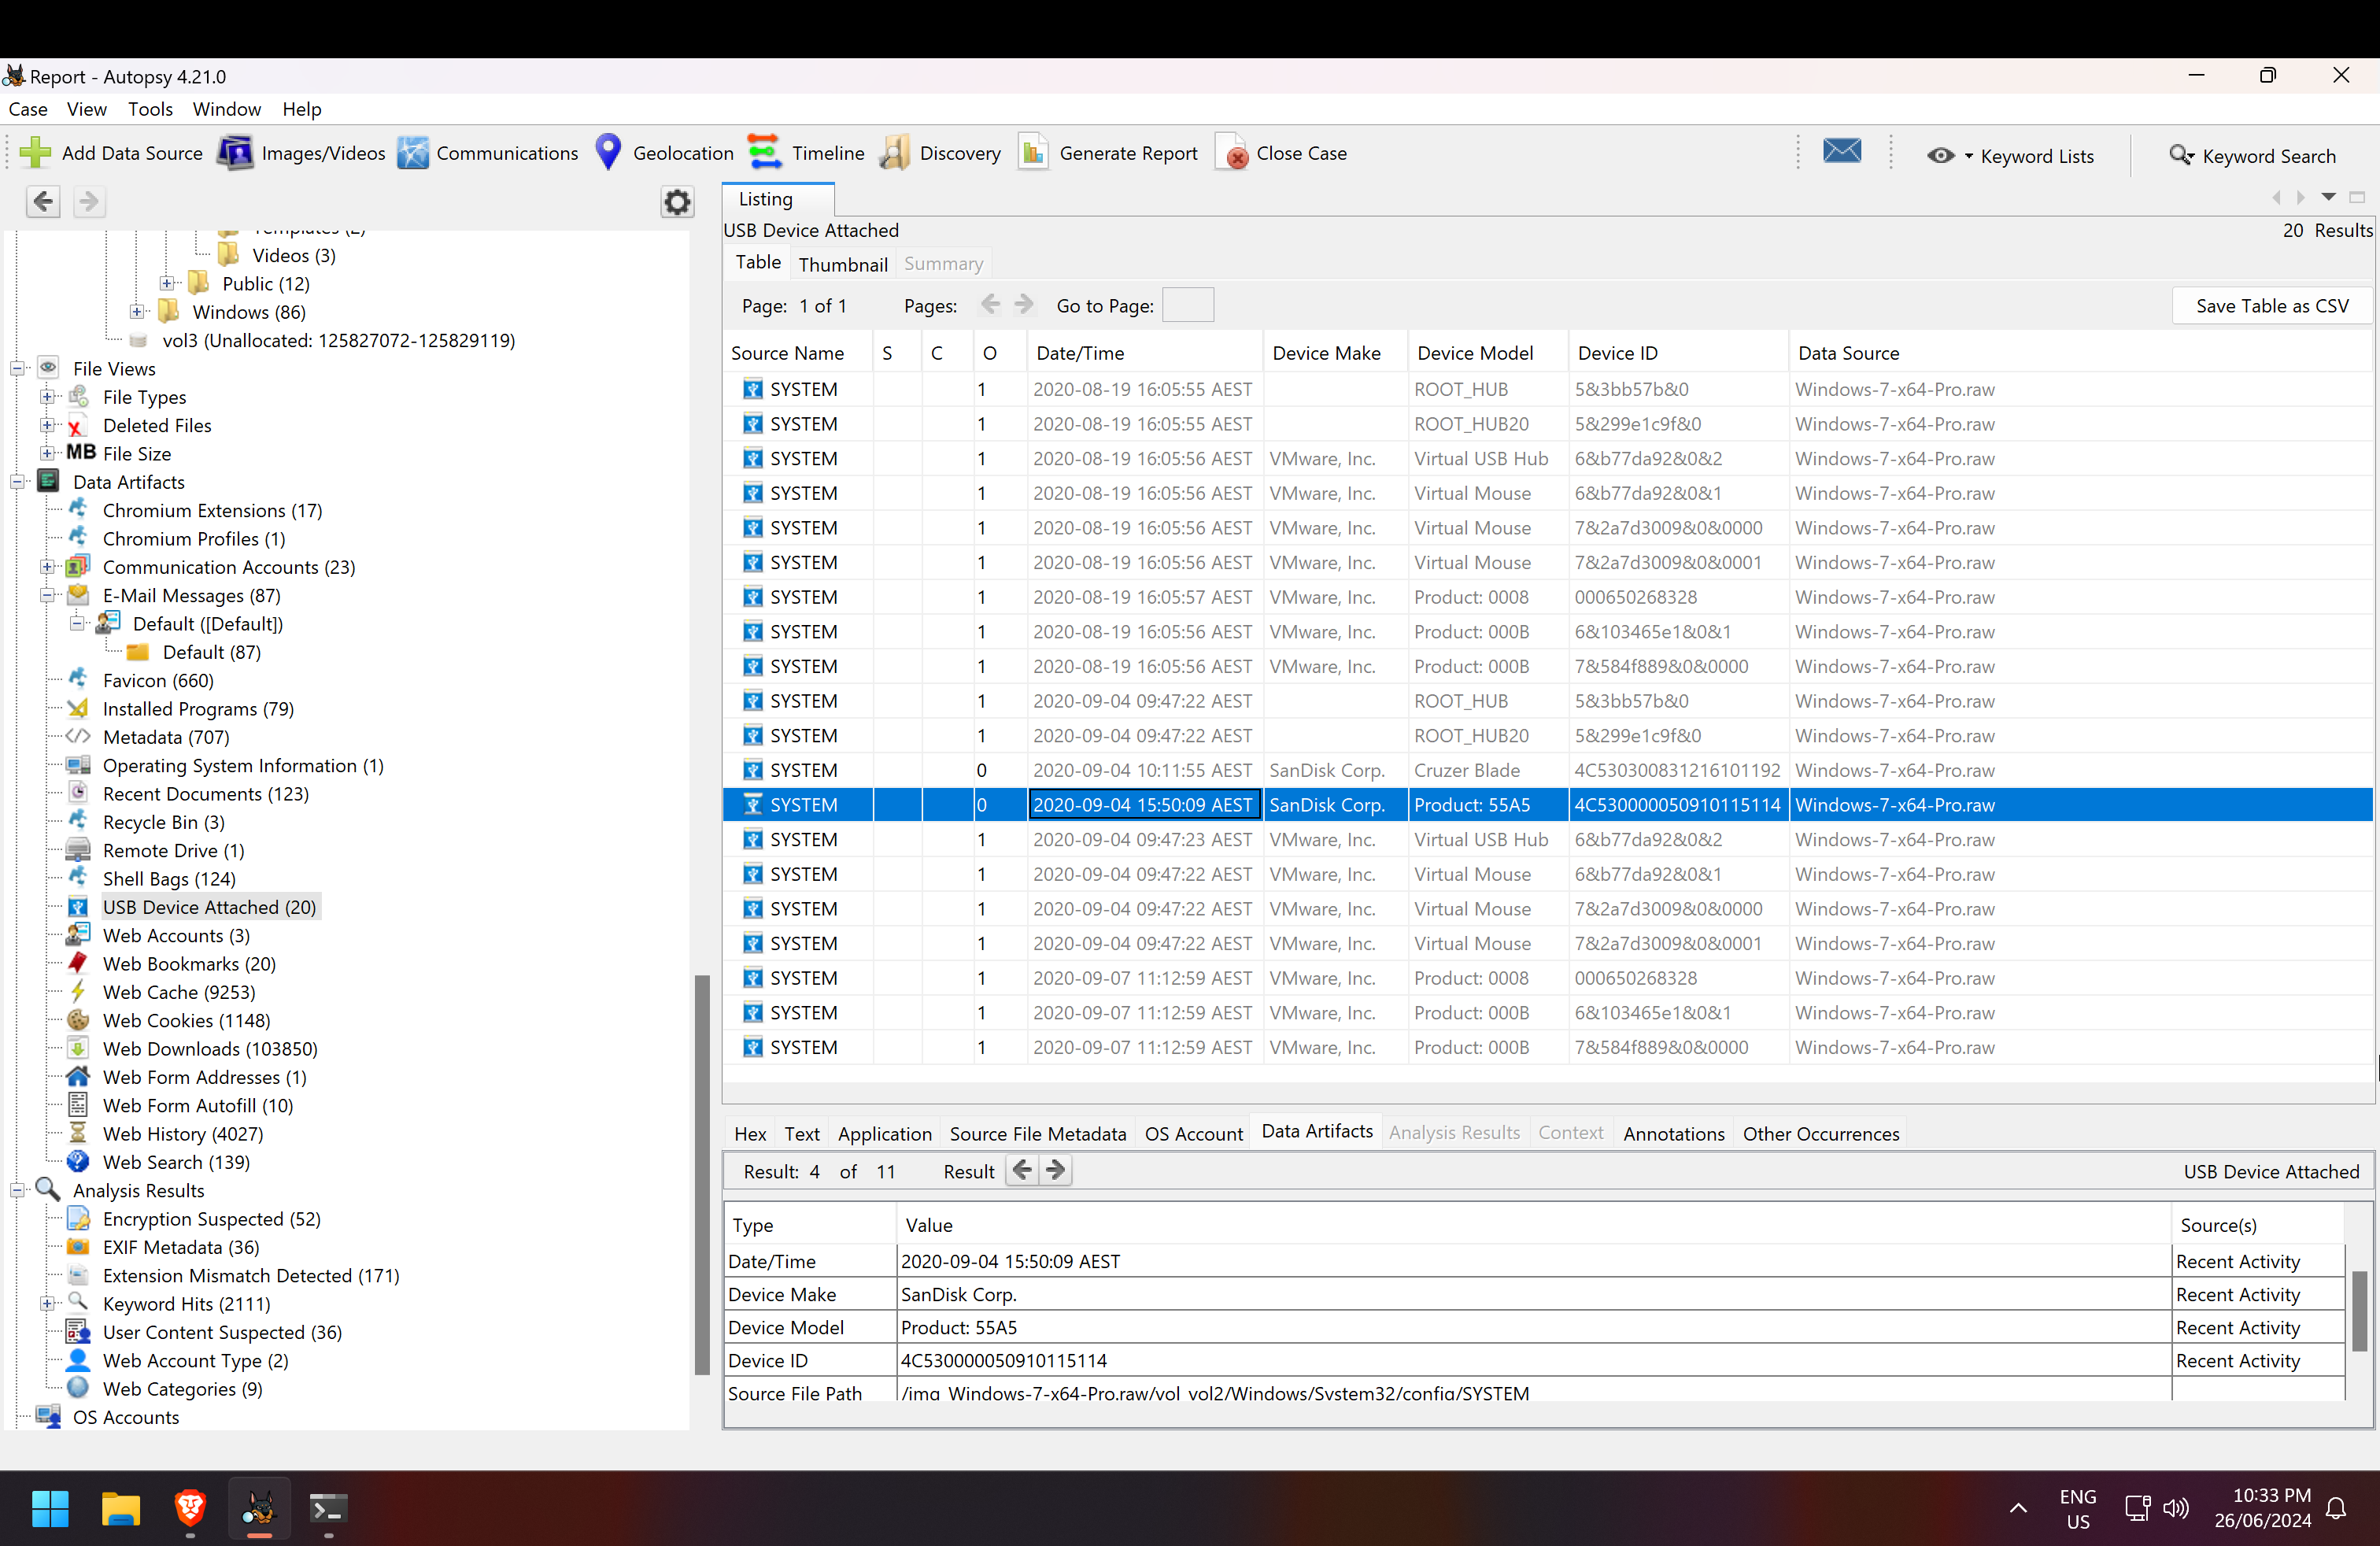
\includegraphics[width=1.0\textwidth]{usb2.png}
    \caption{Attached USB drives}
    \label{fig:usb}
\end{figure}

\begin{figure}[H]
    \centering
    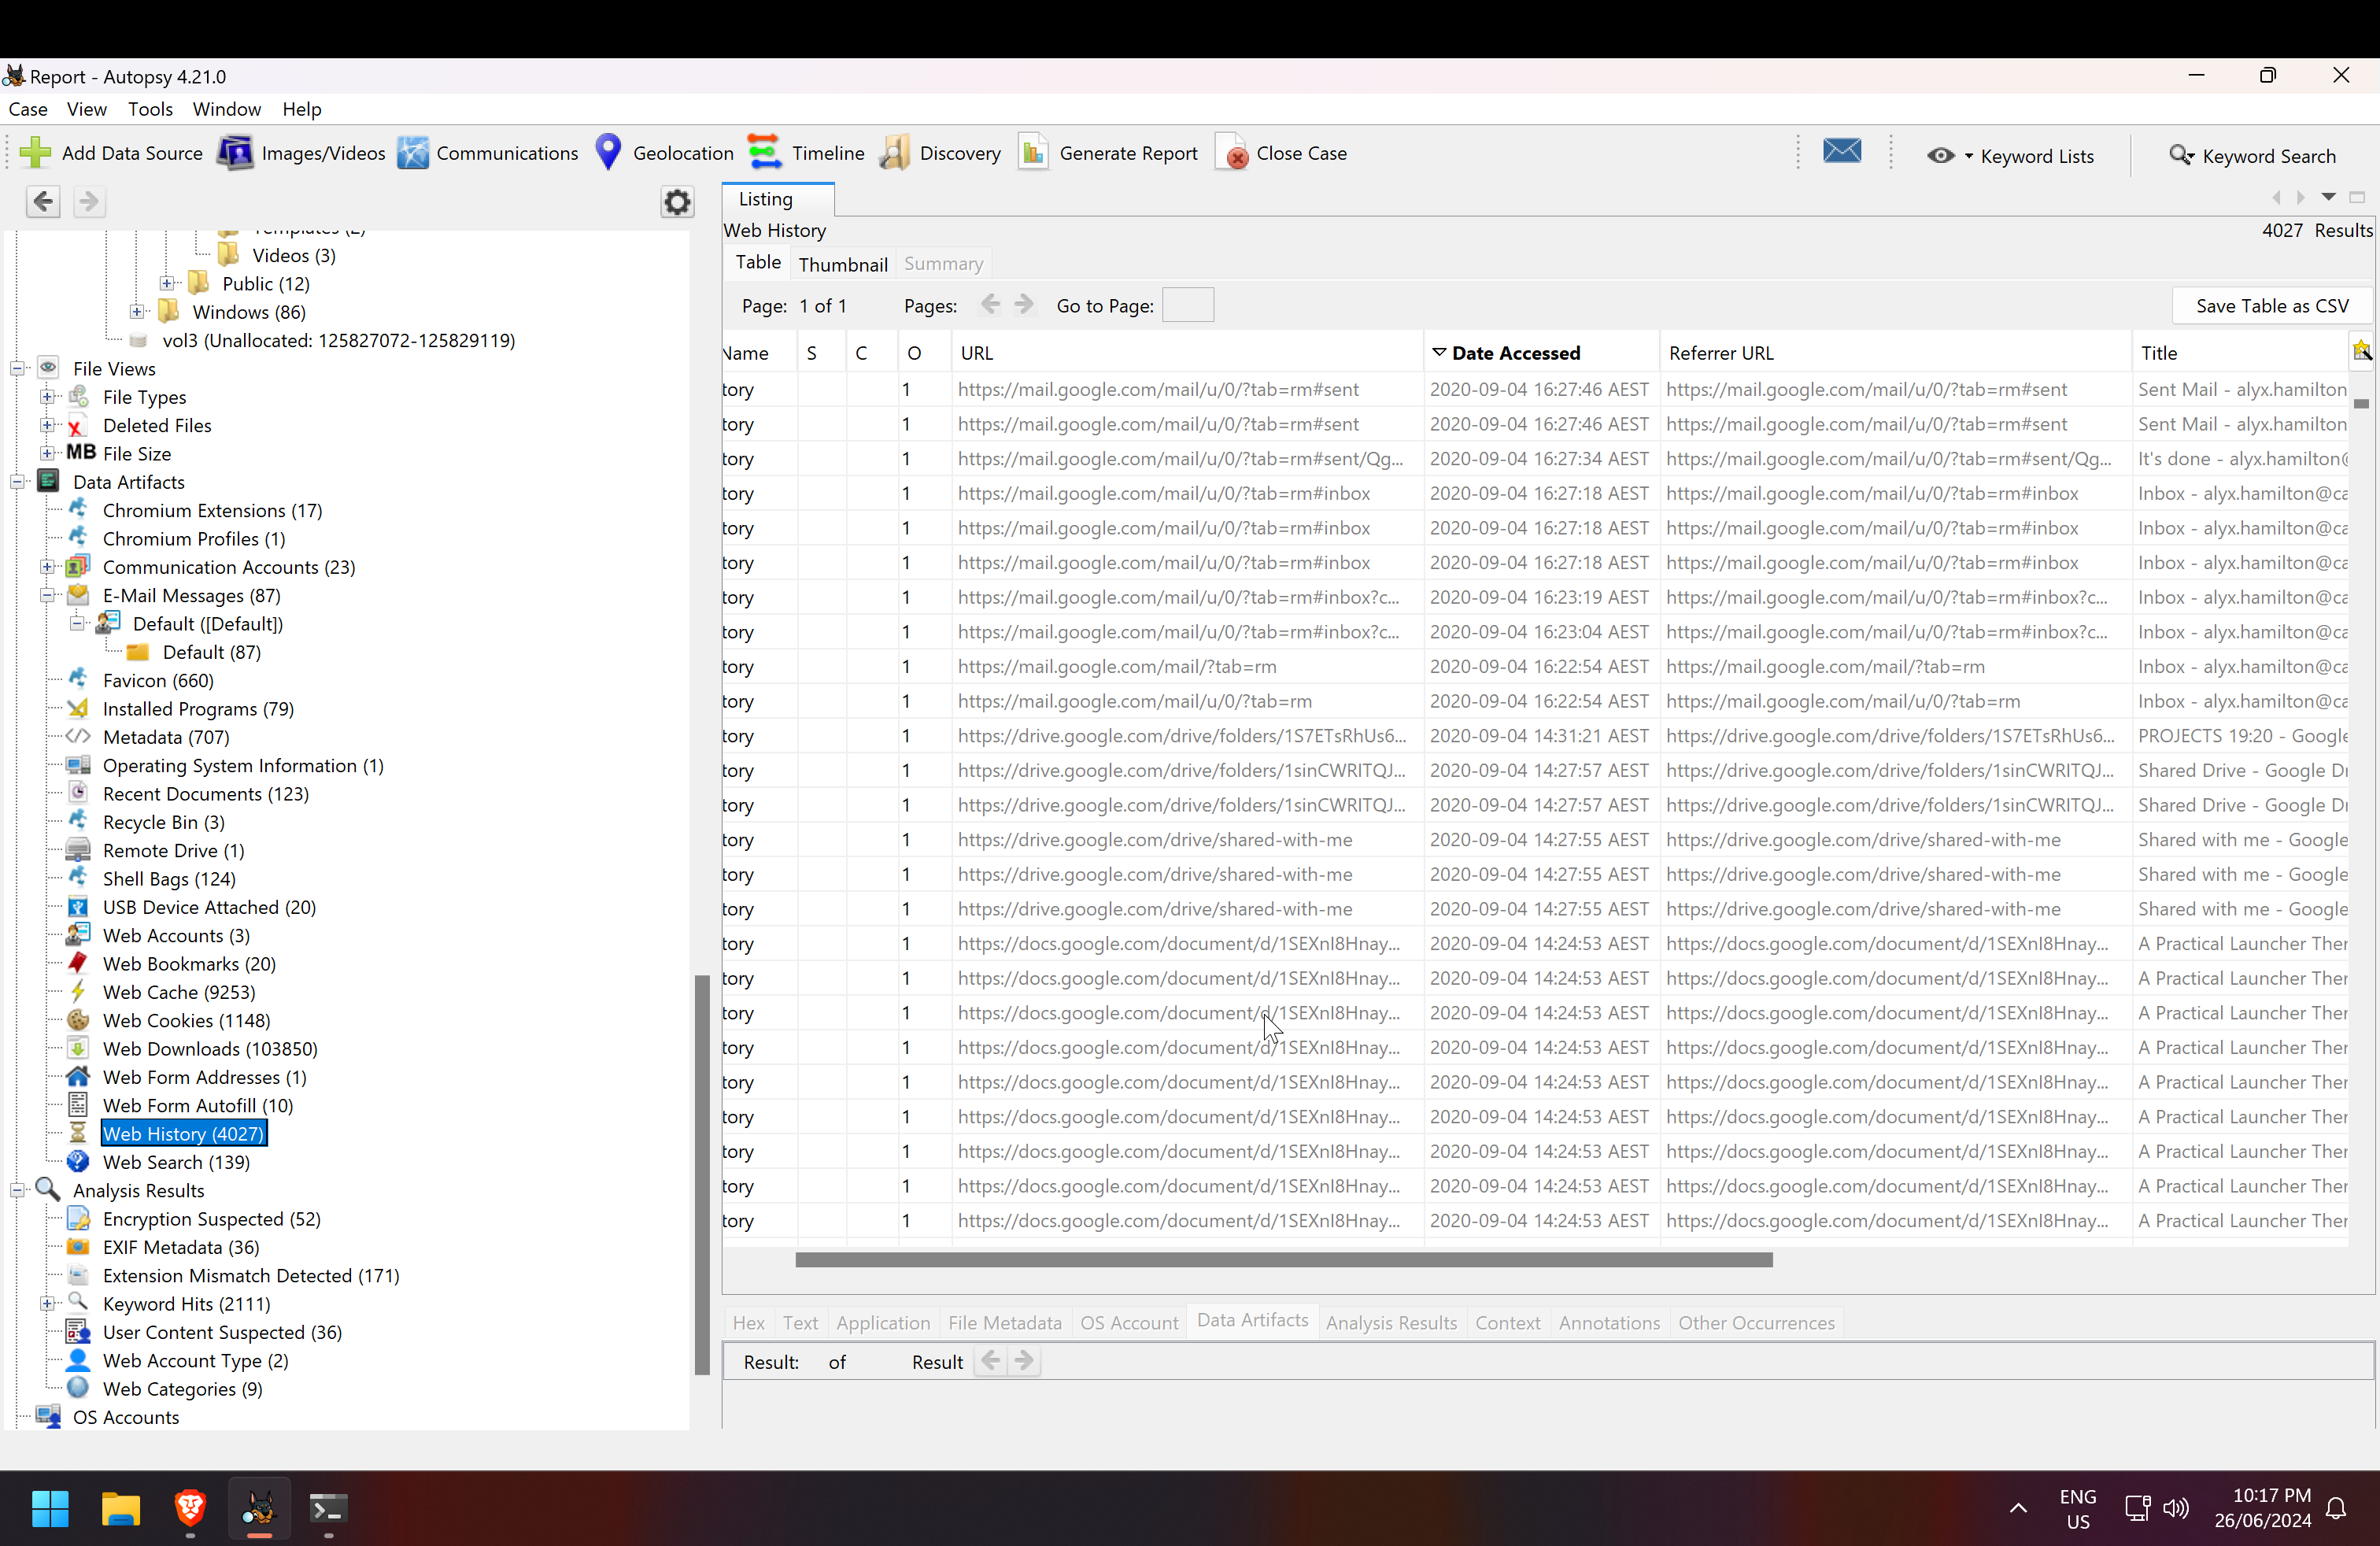
\includegraphics[width=1.0\textwidth]{history1.png}
    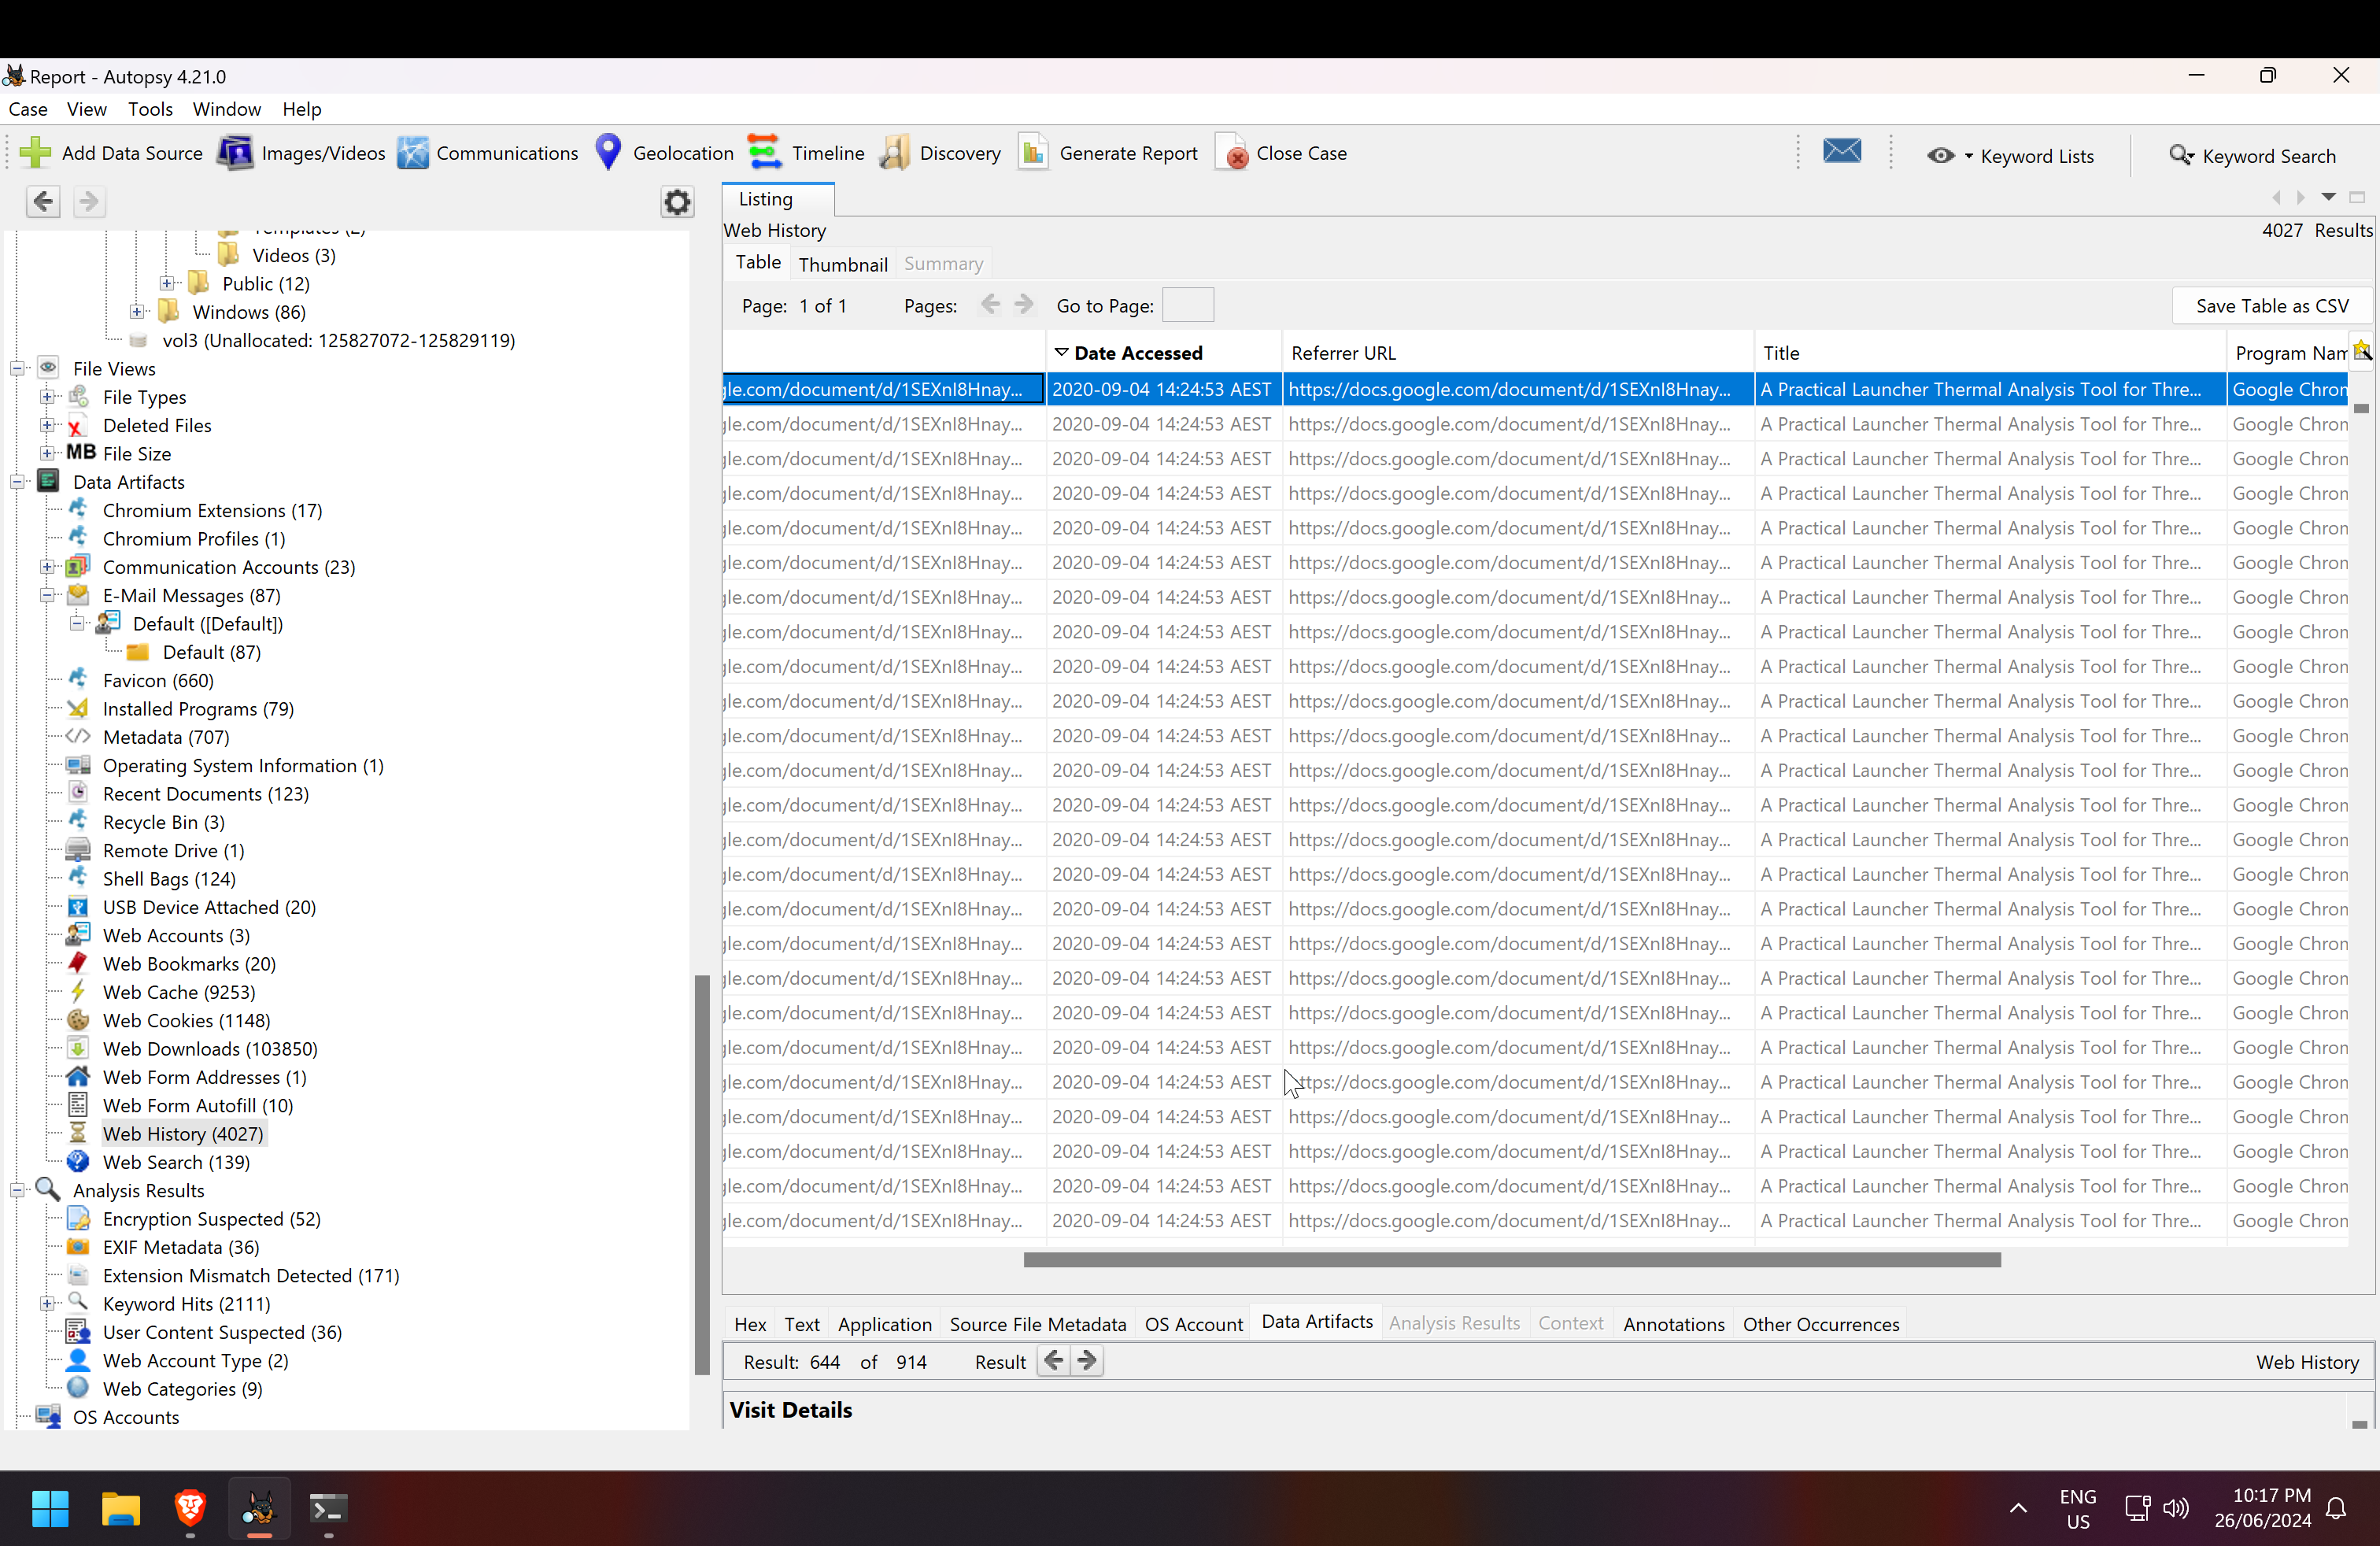
\includegraphics[width=1.0\textwidth]{history2.png}
    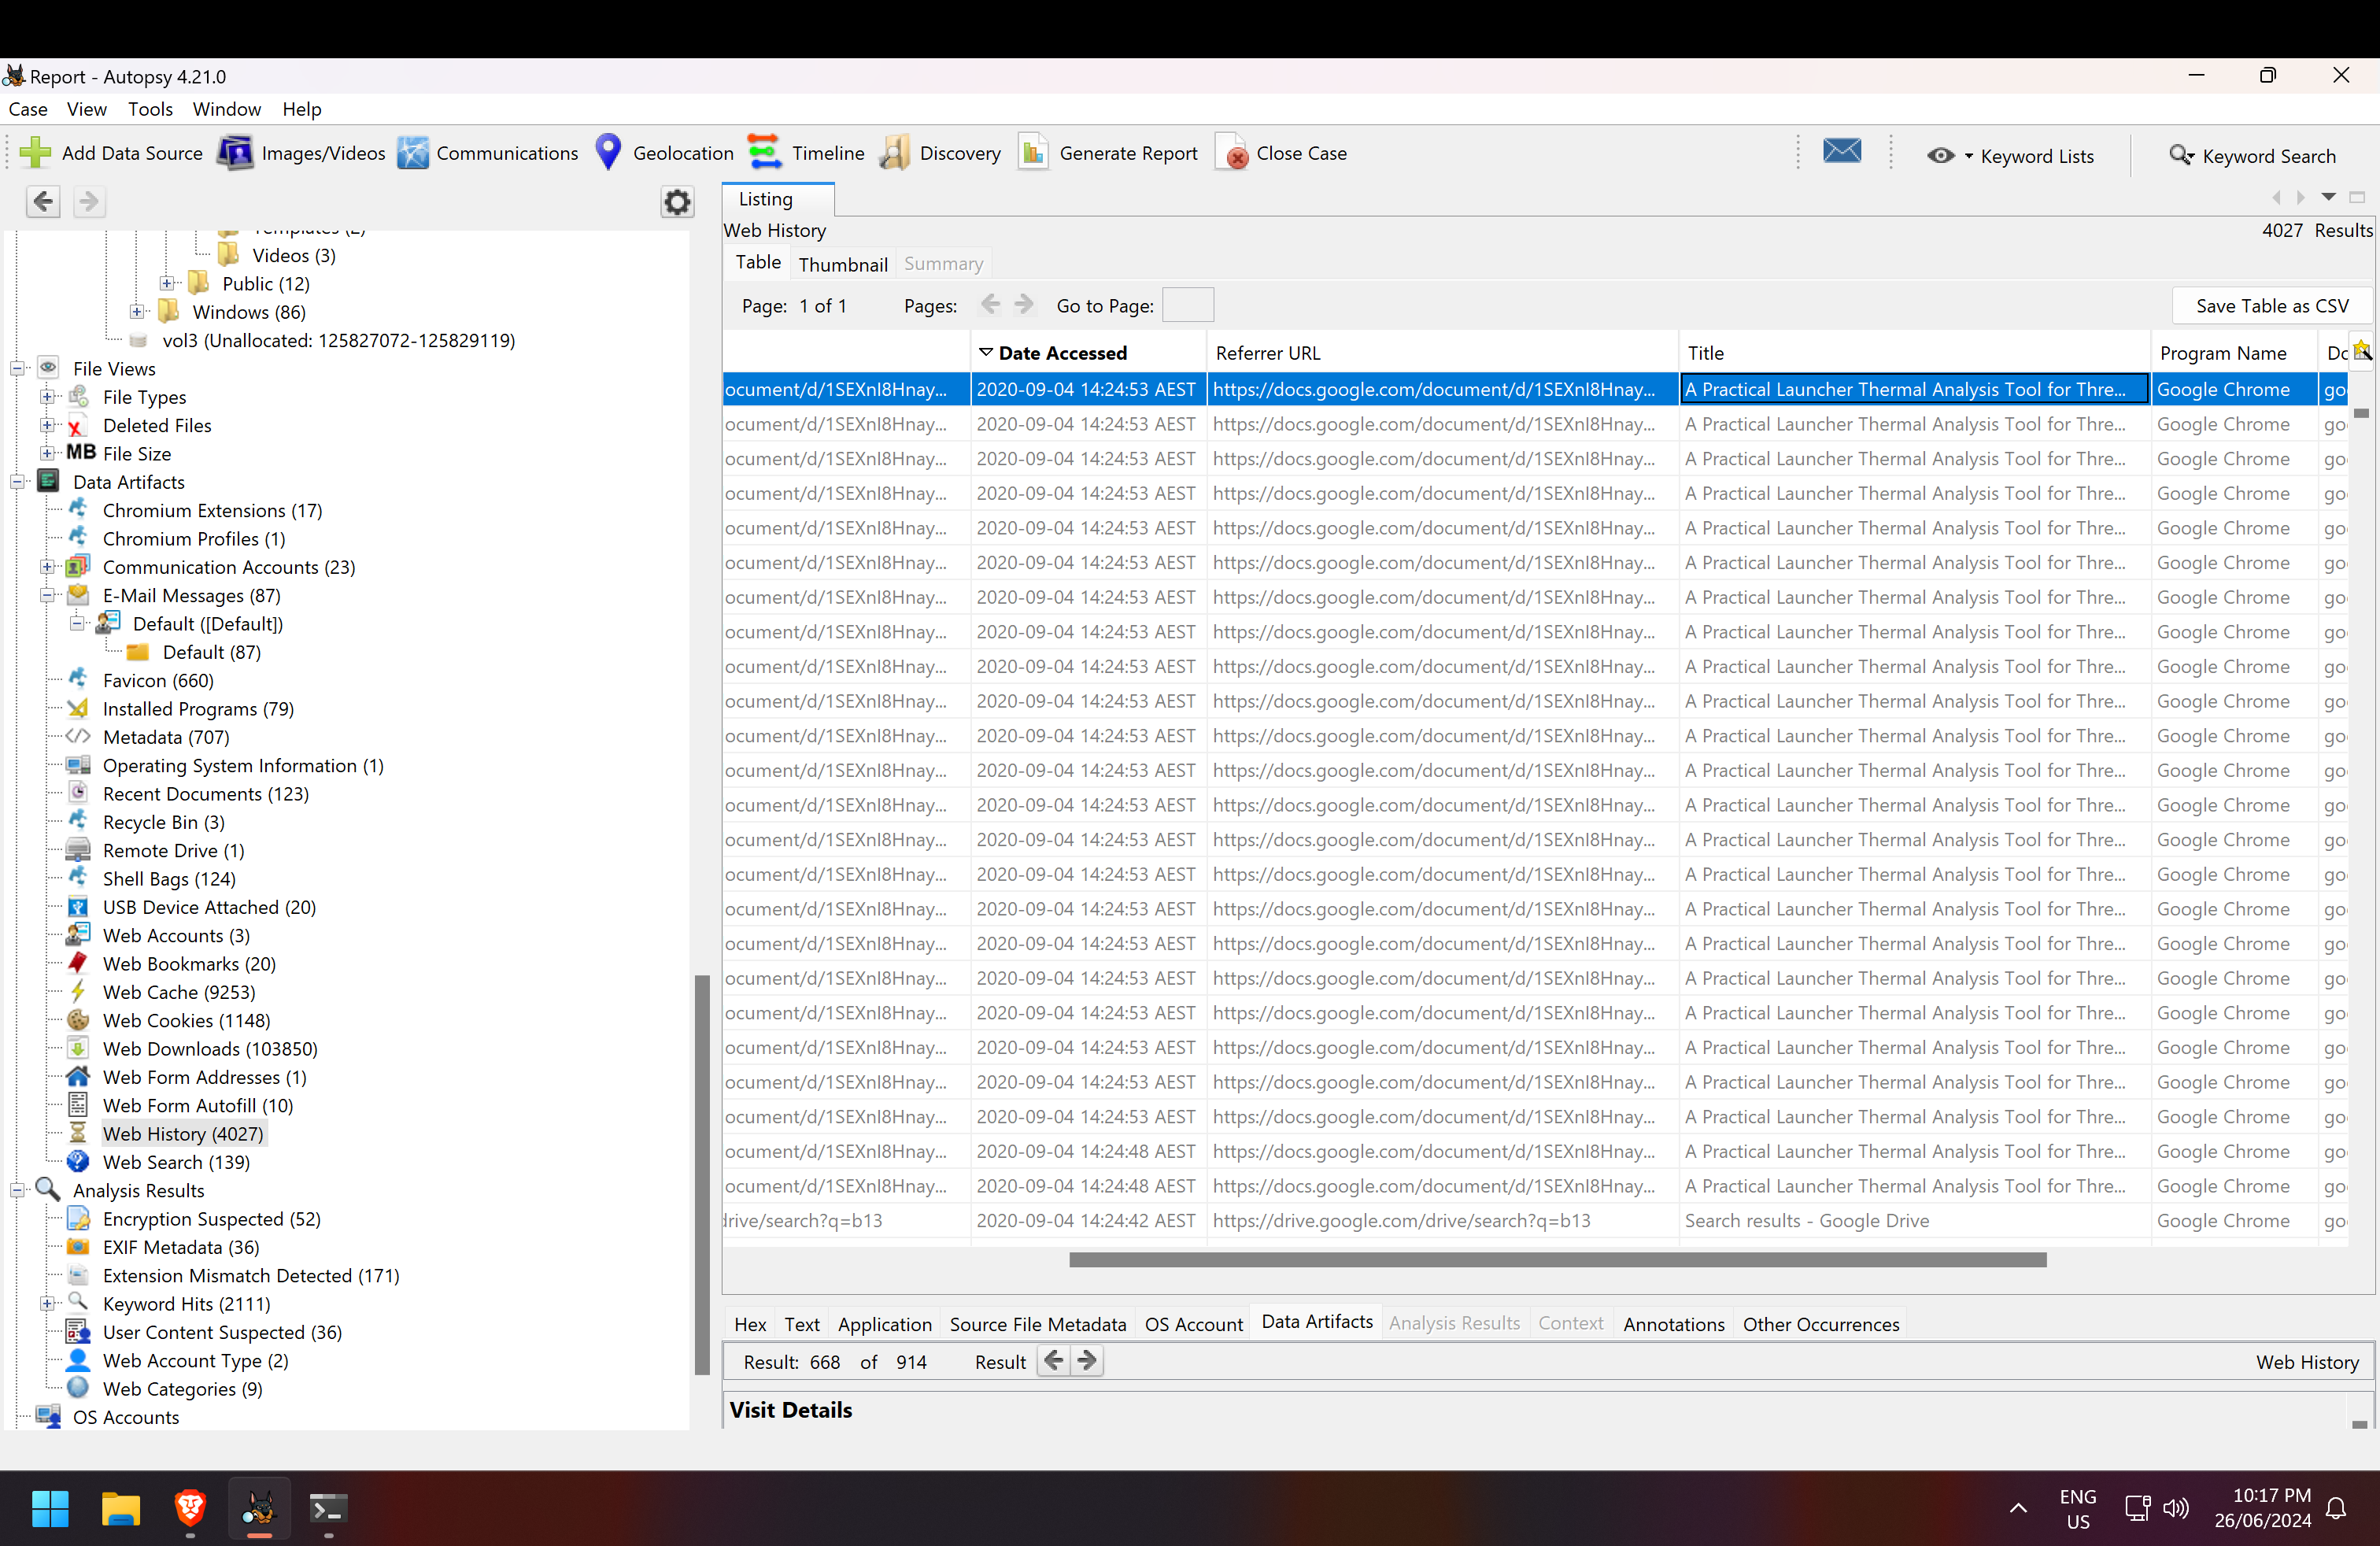
\includegraphics[width=1.0\textwidth]{history3.png}
    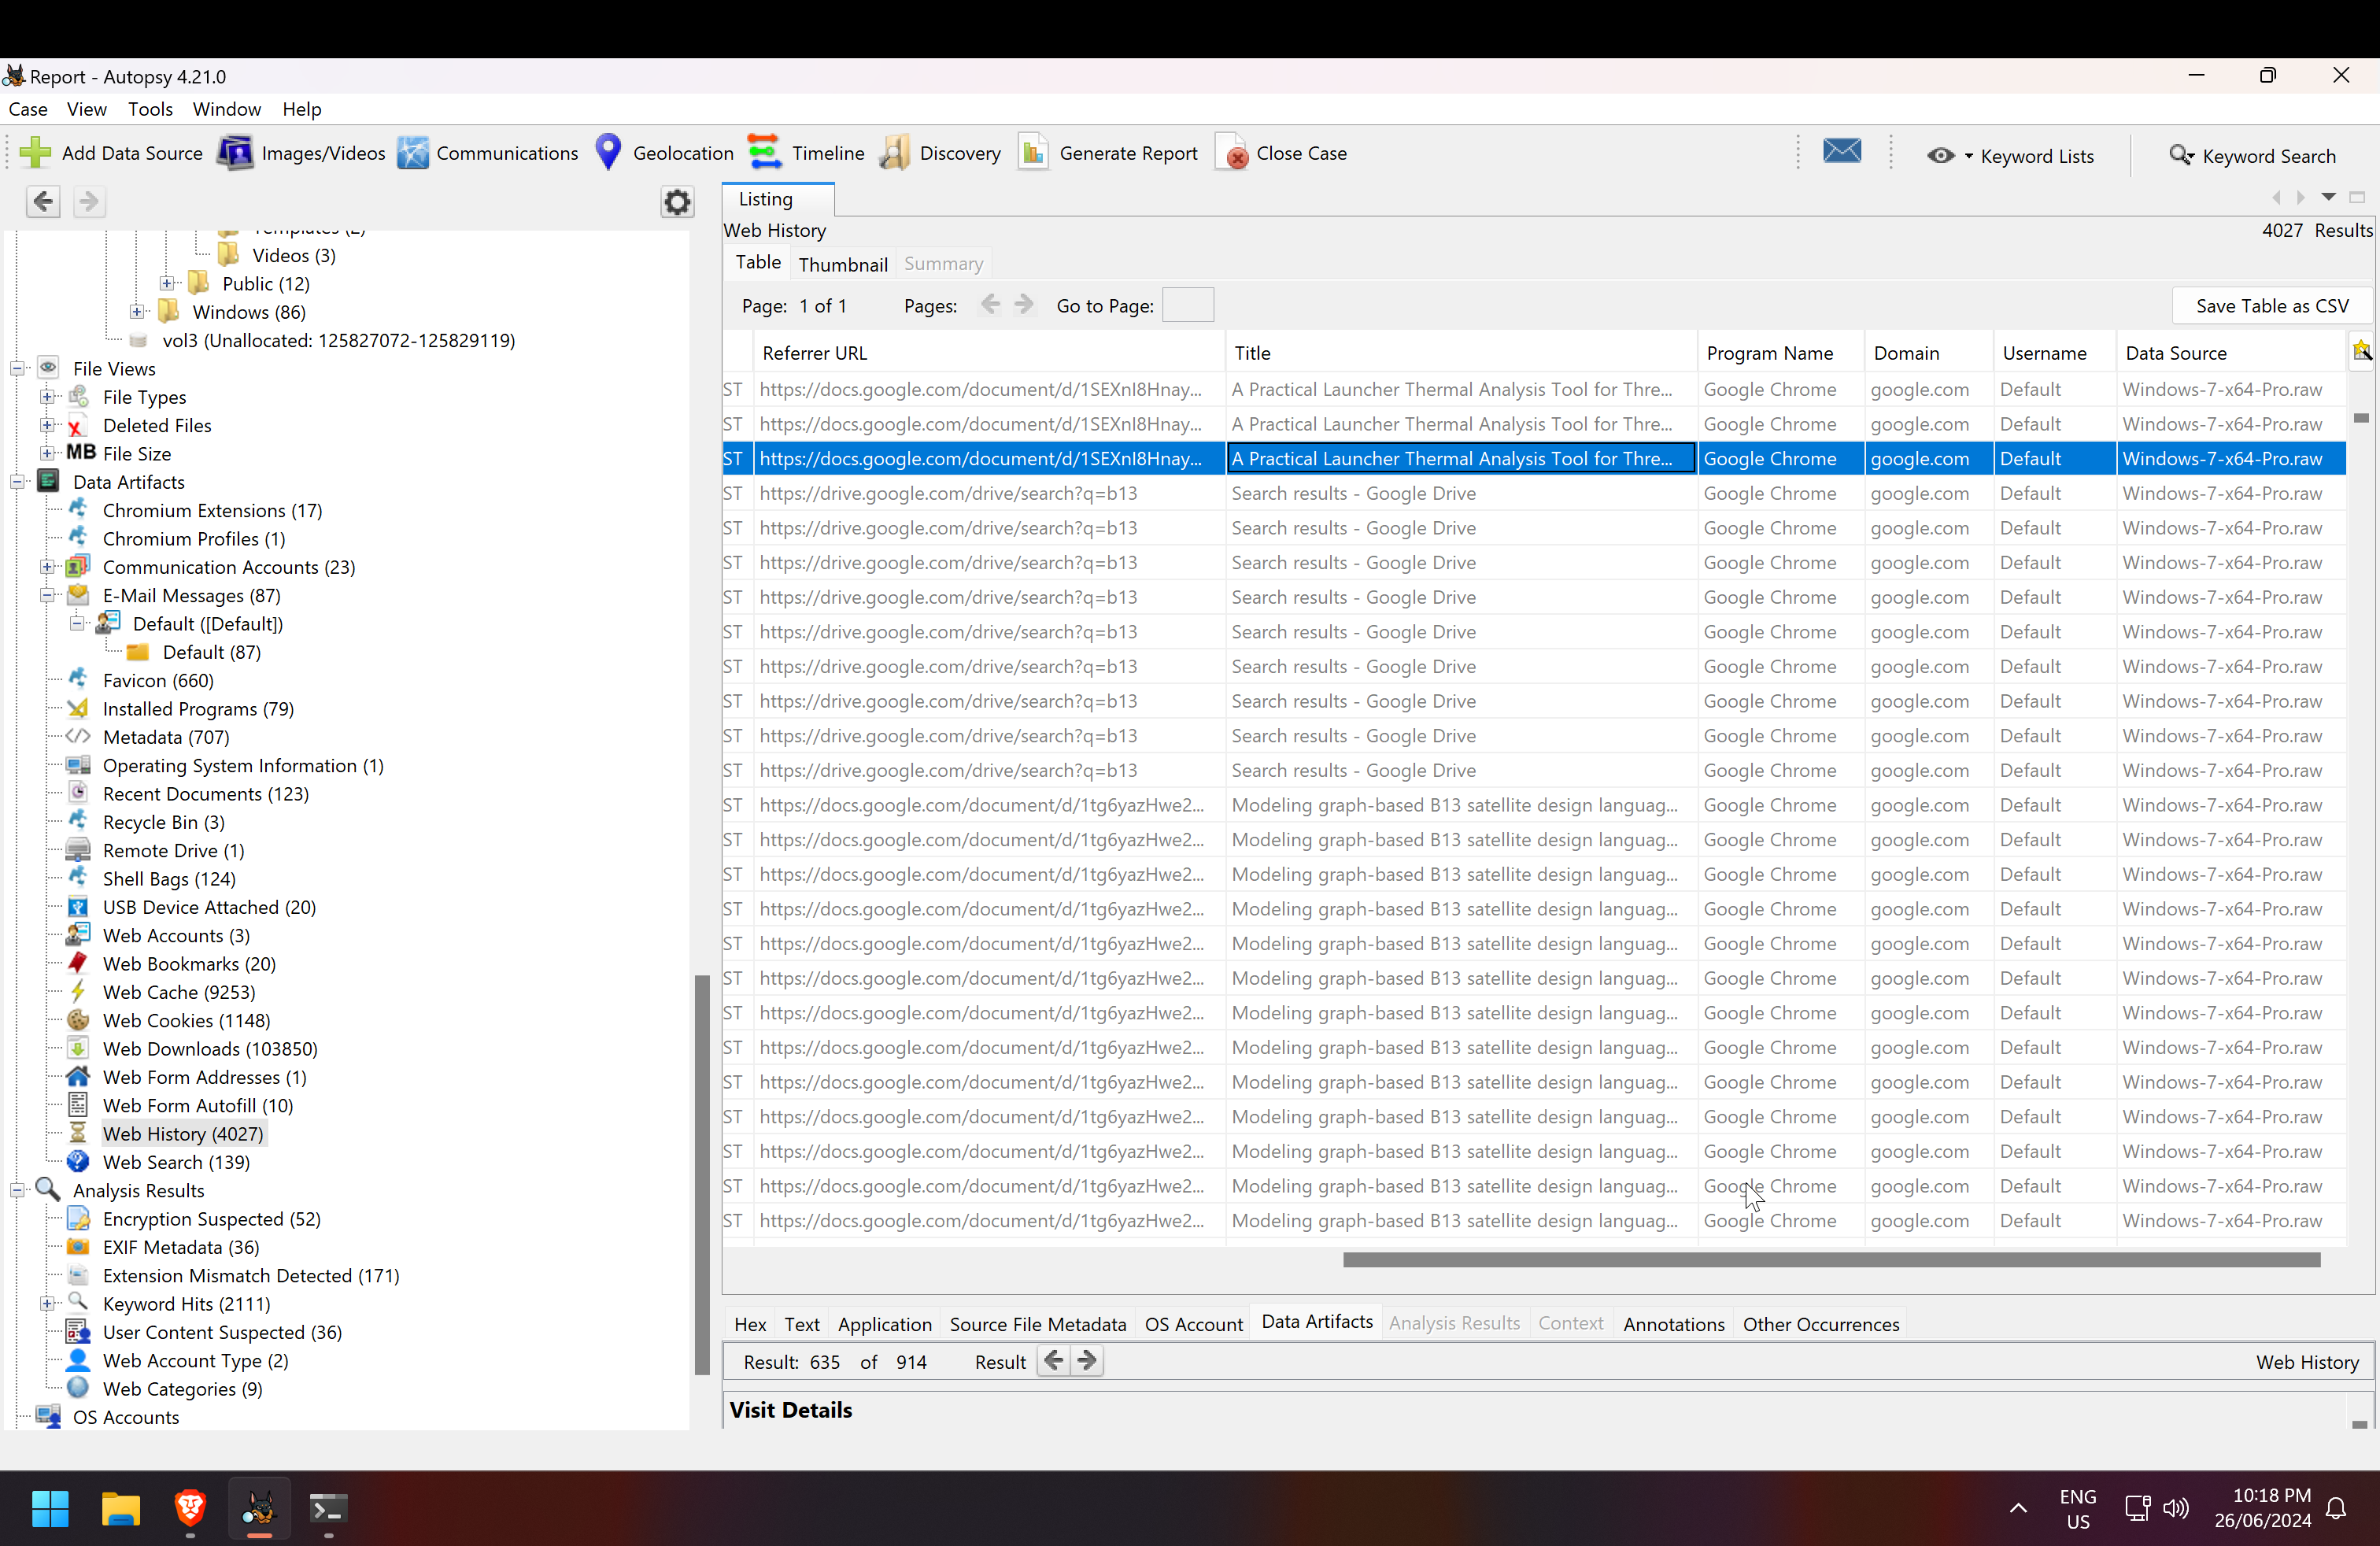
\includegraphics[width=1.0\textwidth]{history4.png}
    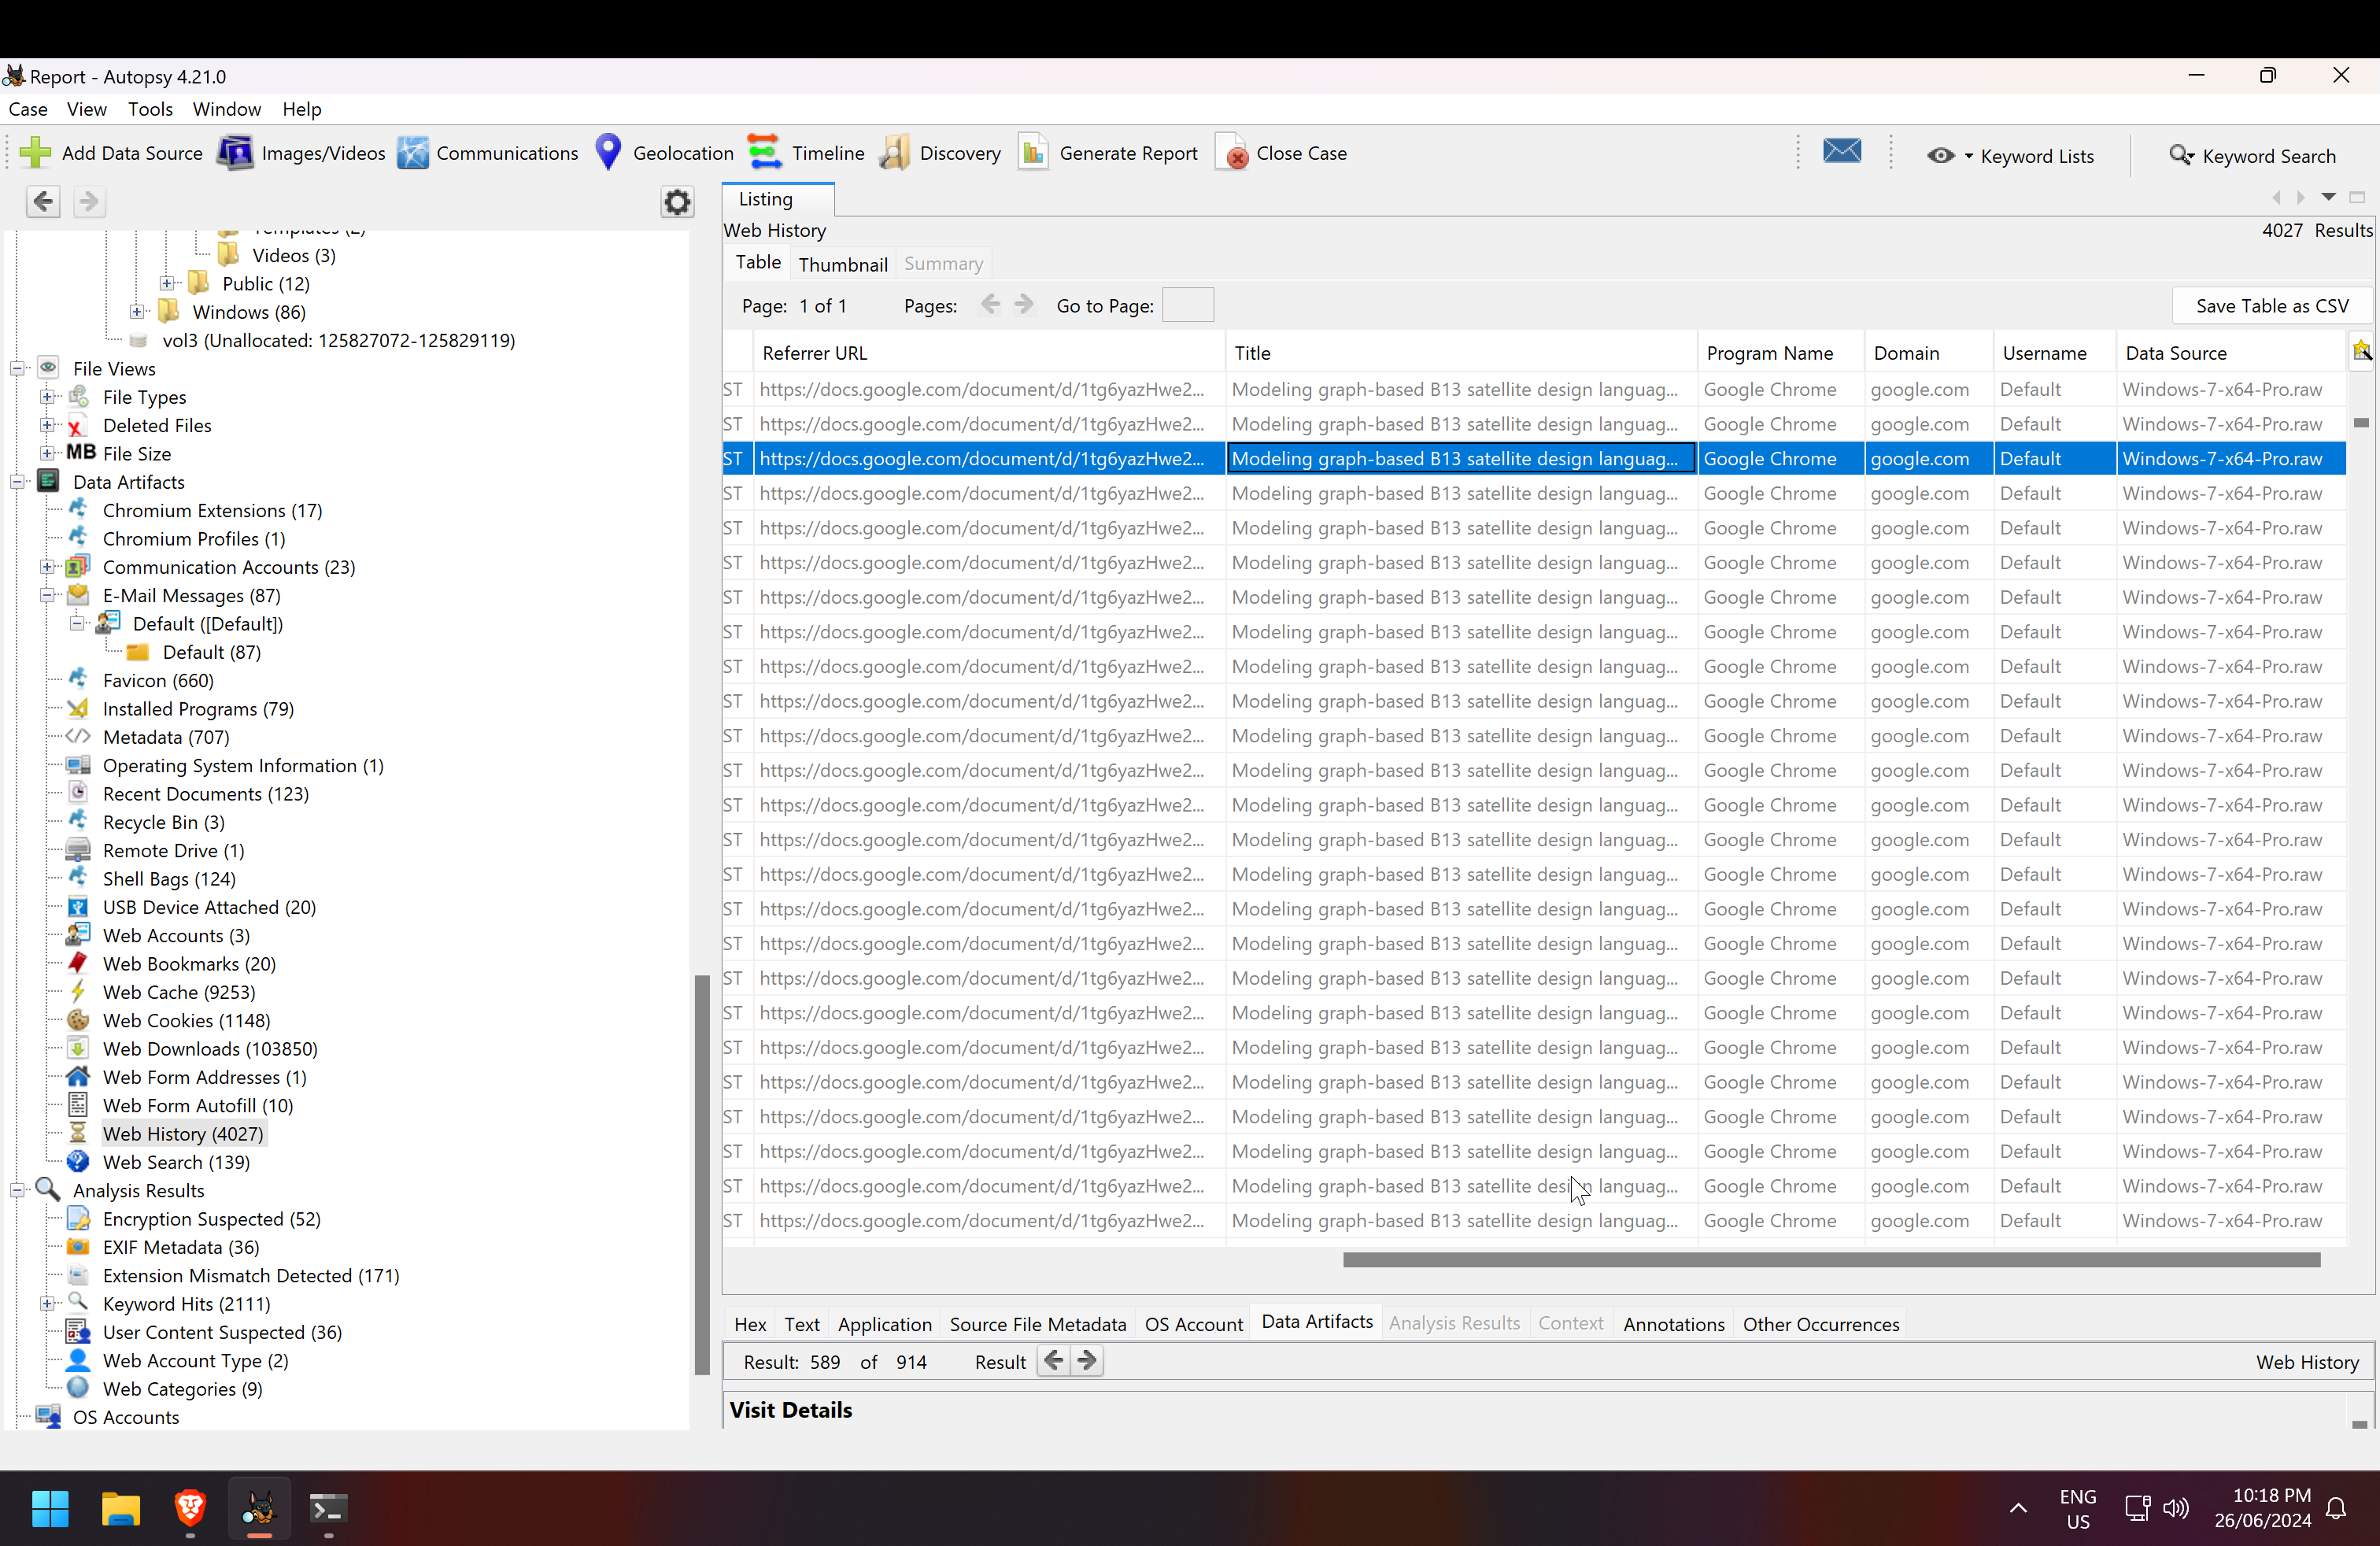
\includegraphics[width=1.0\textwidth]{history5.png}
    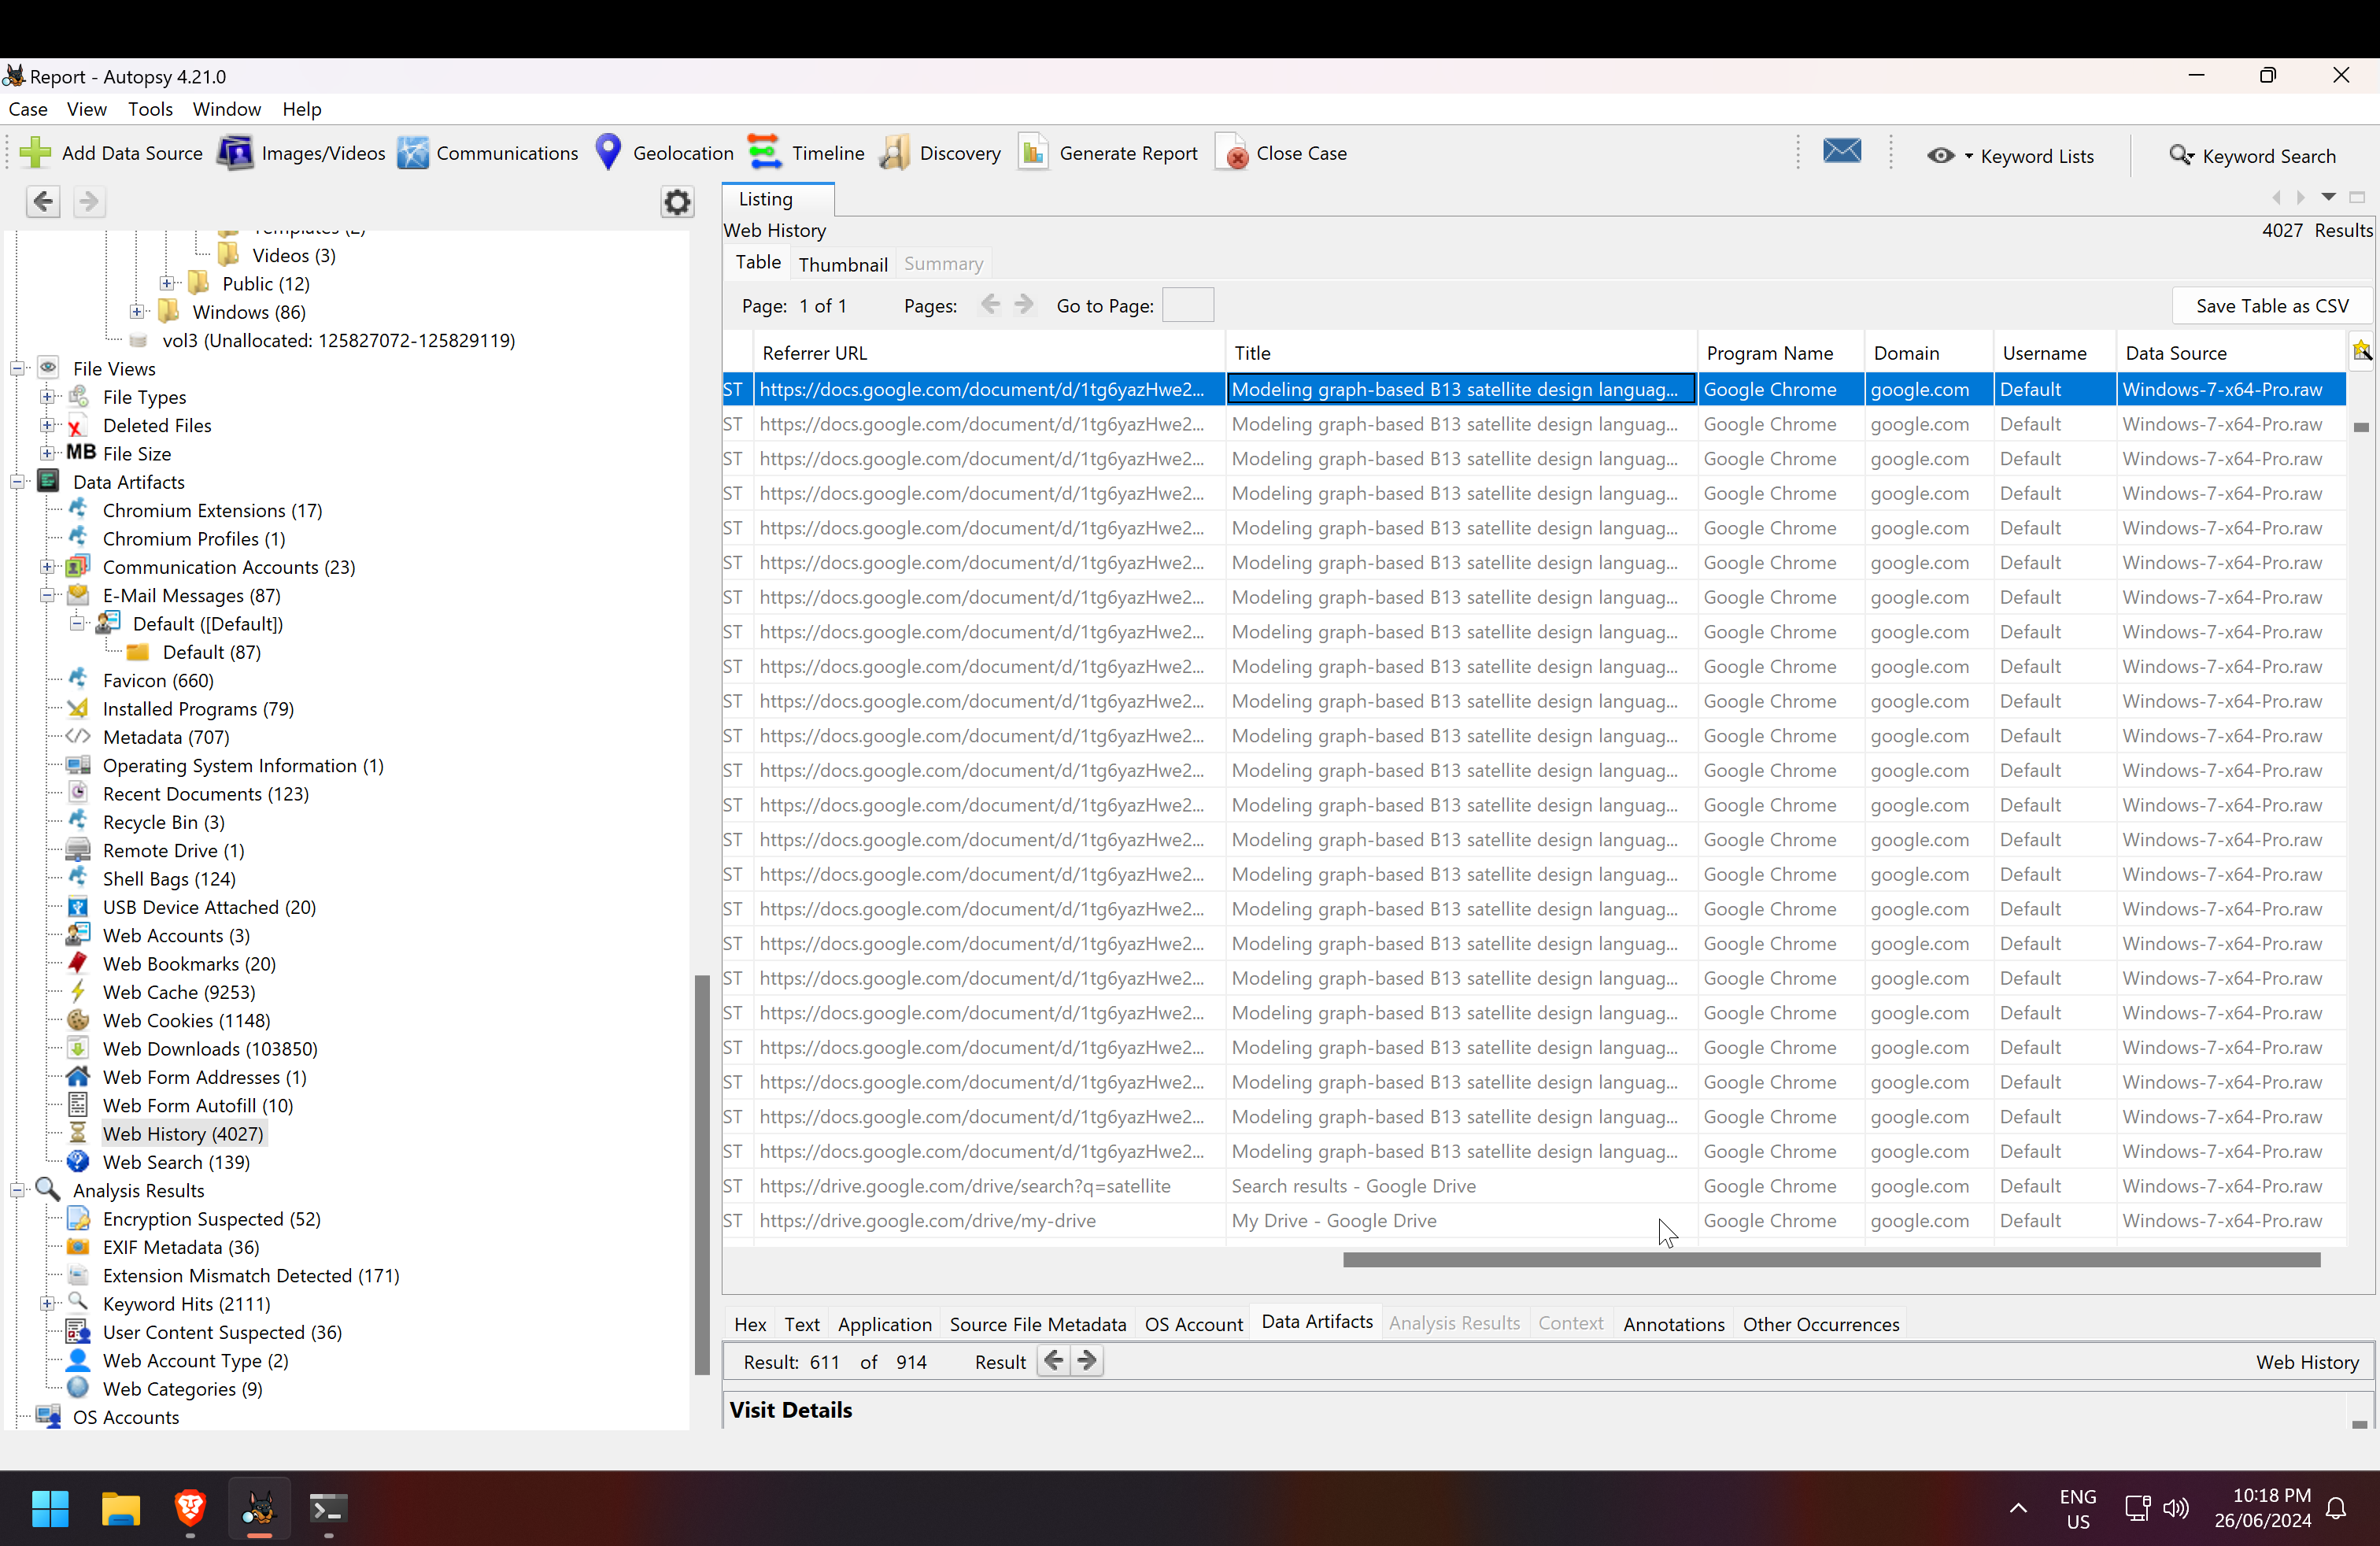
\includegraphics[width=1.0\textwidth]{history6.png}
    \caption{Recent browsing history}
    \label{fig:webhistory}
\end{figure}

\begin{figure}[H]
    \centering
    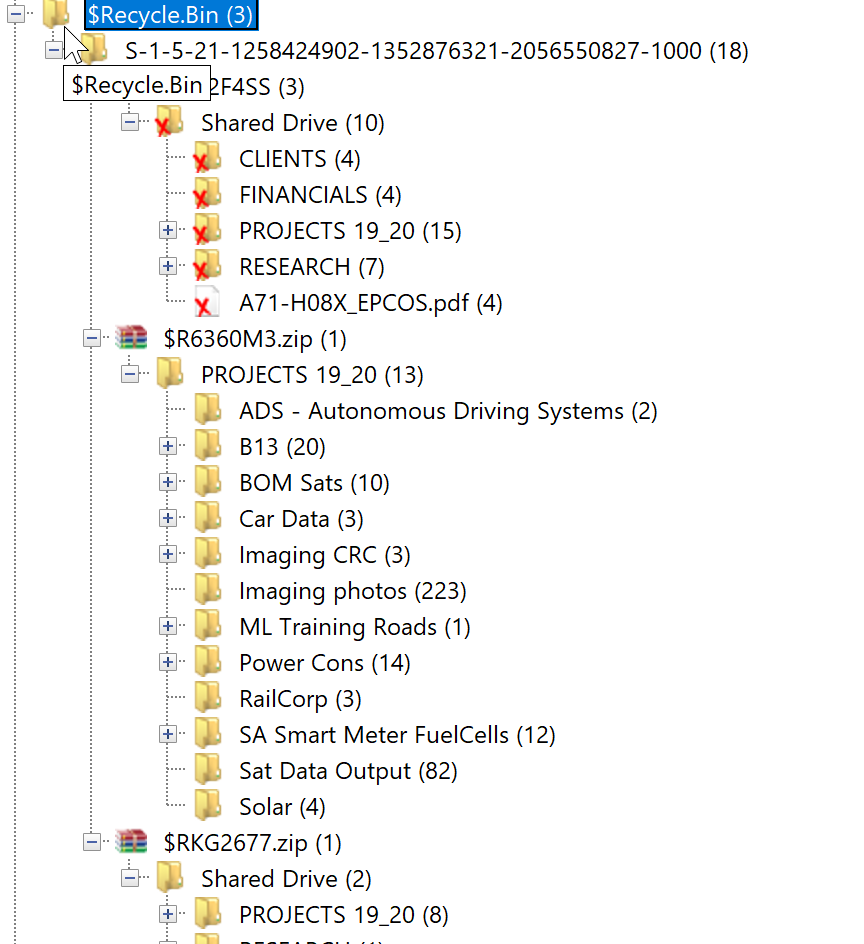
\includegraphics[width=1.0\textwidth]{recycle.png}
    \caption{Recycling bin}
    \label{recycle}
\end{figure}

\begin{figure}[H]
    \centering
    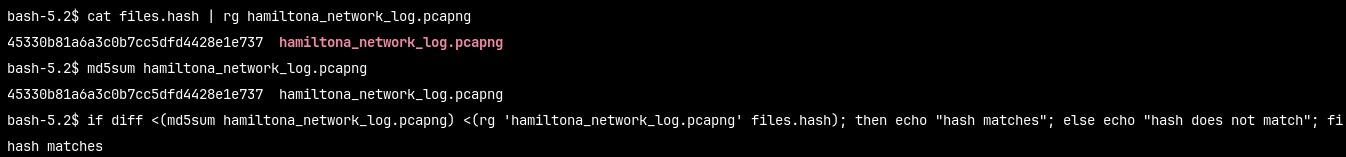
\includegraphics[width=1.0\textwidth]{pcap_verification.png}
    \caption{Cryptographic hash verification of the packet capture file}
    \label{pcap_verification}
\end{figure}

\begin{figure}[H]
    \centering
    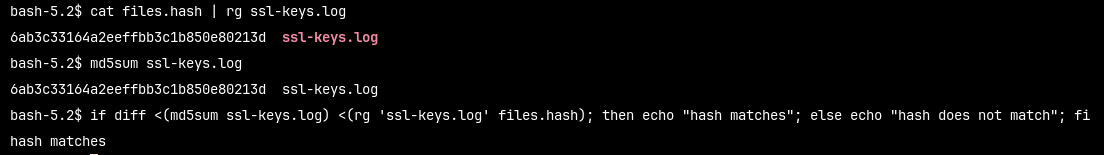
\includegraphics[width=1.0\textwidth]{ssl_key_log_verification.png}
    \caption{Cryptographic hash verification of the SSL key log file}
    \label{ssl_key_log_verification}
\end{figure}

\begin{figure}[H]
    \centering
    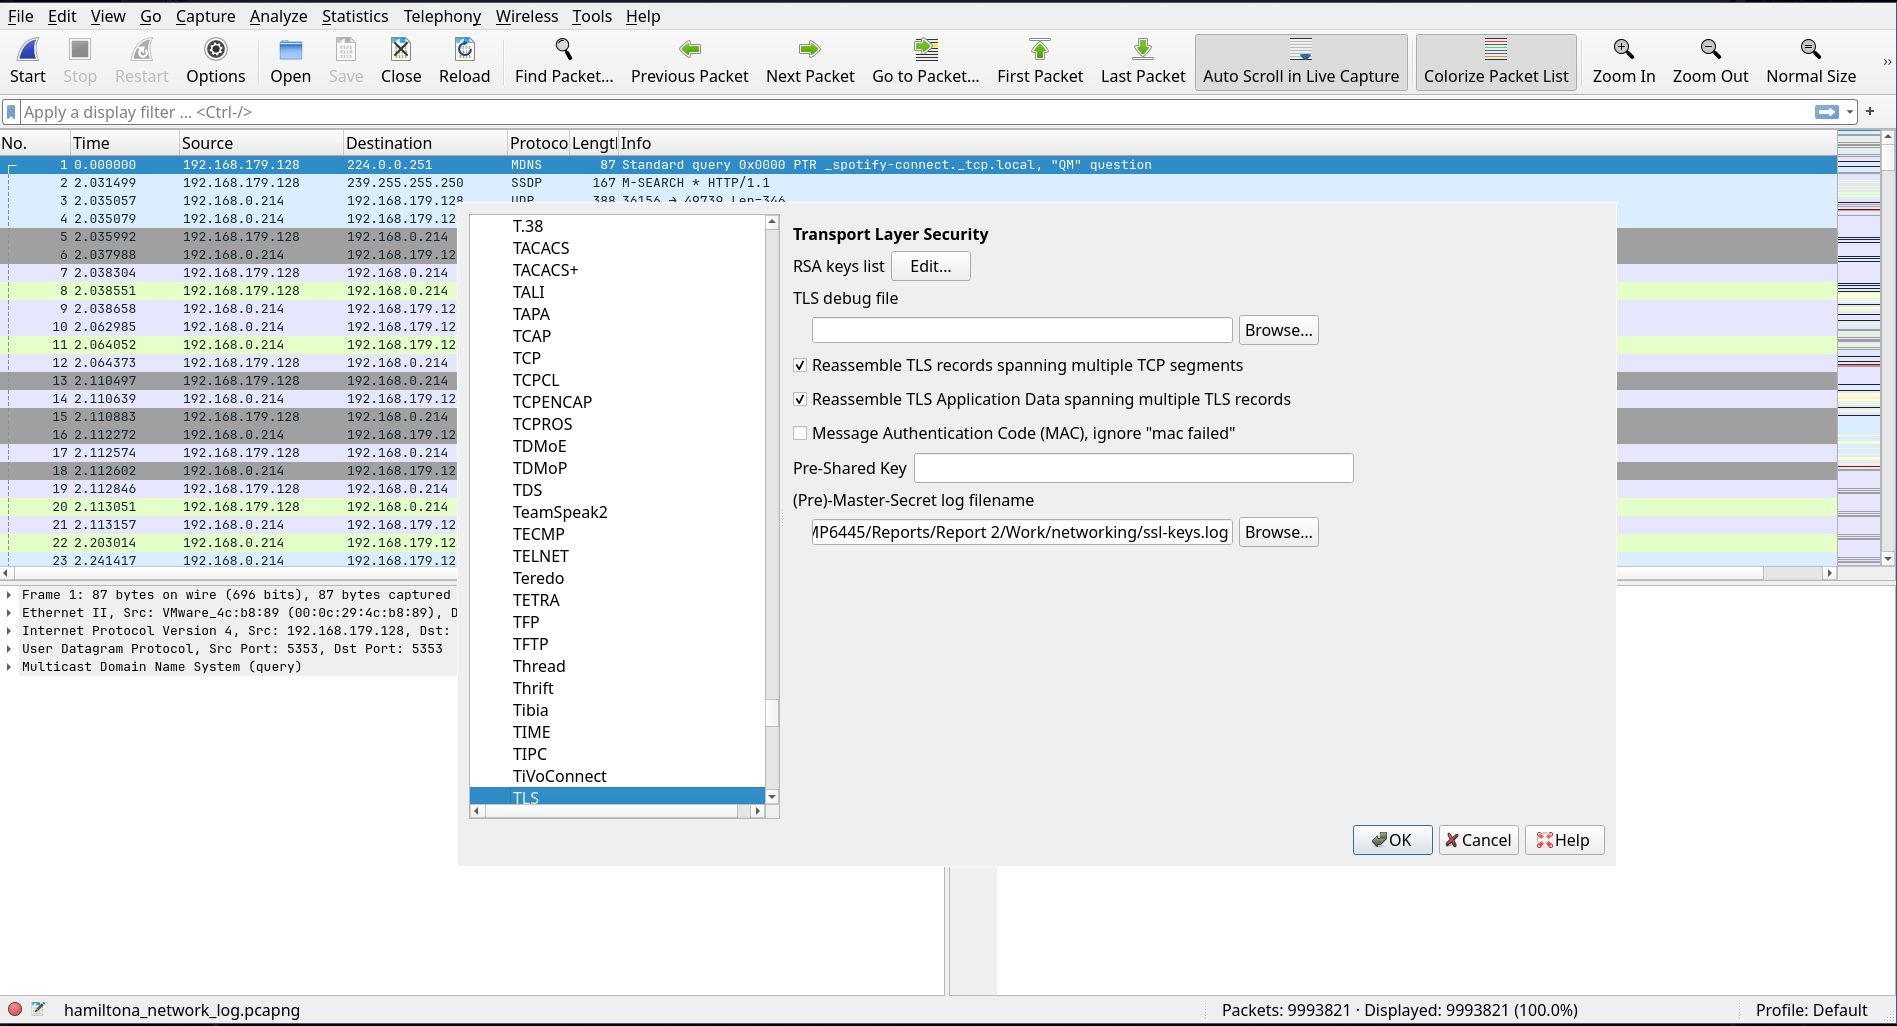
\includegraphics[width=1.0\textwidth]{importing_ssl_key_log.png}
    \caption{Importing the SSL key log to Wireshark}
    \label{importing_ssl_key_log}
\end{figure}

\begin{figure}[H]
    \centering
    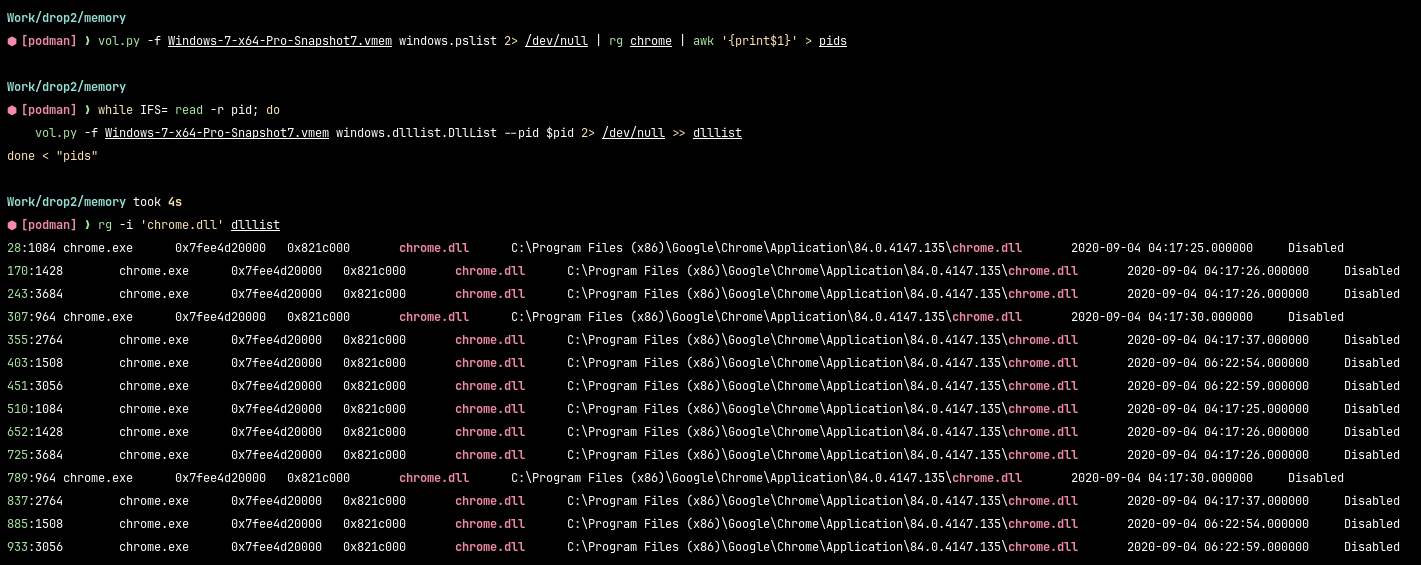
\includegraphics[width=1.0\textwidth]{chrome_version.png}
    \caption{Finding the version of Google Chrome used from the memory dump}
    \label{chrome_version}
\end{figure}

% section Figures (end)

\subsection{Dockerfile for Volatility 3 Environment} % (fold)
\label{sec:Dockerfile for Volatility 3 Environment}
\subsubsection{Dockerfile}
\label{subsubsec:Dockerfile}
\begin{verbatim}
FROM alpine:edge

# Update and install necessary packages
RUN apk update && apk upgrade && apk add --no-cache \
    python3 \
    7zip \
    shadow \
    curl \
    git \
    tmux \
    neovim \
    starship \
    clang \
    zsh \
    bat \
    eza \
    fzf \
    ripgrep \
    fd \
    bind-tools \
    py3-virtualenv \
    termshark \
    traceroute \
    neomutt

# Add a new user
RUN adduser -D COMP6845
RUN usermod -aG wireshark COMP6845
RUN chsh -s /bin/zsh COMP6845

USER COMP6845
WORKDIR /home/COMP6845

# Clone necessary repositories
RUN git clone https://github.com/tmux-plugins/tpm /home/COMP6845/.local/share/tmux/plugins/tpm
RUN git clone https://github.com/zsh-users/zsh-syntax-highlighting.git /home/COMP6845/.local/share/zsh/zsh-syntax-highlighting
RUN git clone https://github.com/zsh-users/zsh-autosuggestions /home/COMP6845/.local/share/zsh/zsh-autosuggestions
RUN git clone https://github.com/Aloxaf/fzf-tab /home/COMP6845/.local/share/zsh/fzf-tab

# Set up volatility
RUN mkdir -p /home/COMP6845/.local/bin
WORKDIR /home/COMP6845/.local/bin
RUN python3 -m venv volatility
RUN ./volatility/bin/pip install --upgrade pip
RUN ./volatility/bin/pip install volatility3

WORKDIR /home/COMP6845
RUN echo "alias 'vol.py'='/home/COMP6845/.local/bin/volatility/bin/vol'" >> .zshrc

# Create Mail directory and copy mbox files
RUN mkdir -p /home/COMP6845/Mail
COPY --chown=COMP6845:COMP6845 Emails/Harris/all.mbox /home/COMP6845/Mail/harris.mbox
COPY --chown=COMP6845:COMP6845 Emails/Hamilton/all.mbox /home/COMP6845/Mail/hamilton.mbox

# Configure NeoMutt
RUN echo 'set mbox_type=mbox' >> /home/COMP6845/.neomuttrc
RUN echo 'set folder=~/Mail' >> /home/COMP6845/.neomuttrc
RUN echo 'mailboxes ~/Mail/hamilton.mbox ~/Mail/harris.mbox' >> /home/COMP6845/.neomuttrc
RUN echo 'set spoolfile=~/Mail/hamilton.mbox' >> /home/COMP6845/.neomuttrc

CMD ["zsh"]
\end{verbatim}

\subsubsection{zshrc}
\label{subsubsec:zshrc}

\begin{verbatim}
# Lines configured by zsh-newuser-install
HISTFILE=~/.histfile
HISTSIZE=1000
SAVEHIST=1000
bindkey -e
# End of lines configured by zsh-newuser-install
# The following lines were added by compinstall
zstyle :compinstall filename '/home/COMP3141/.zshrc'

autoload -Uz compinit
compinit
# End of lines added by compinstall

alias vim=nvim
alias v=nvim

alias cat=bat

alias ls='eza --icons'
alias ll='eza --icons -l'
alias la='eza --icons -la'

# Plugins
source ~/.local/share/zsh/zsh-syntax-highlighting/zsh-syntax-highlighting.zsh
source ~/.local/share/zsh/zsh-autosuggestions/zsh-autosuggestions.zsh
source ~/.local/share/zsh/fzf-tab/fzf-tab.plugin.zsh

# Start starship
# ~/.zshrc
eval "$(starship init zsh)"
\end{verbatim}

\subsubsection{Instructions for use}

Install and set up Docker or Podman. Then:

\begin{enumerate}
    \item Create a new, empty directory and change into said directory.
    \item Copy the contents of Section~\ref{subsubsec:Dockerfile} into a file named \texttt{Dockerfile} in the current working directory.
    \item Copy the contents of Section~\ref{subsubsec:zshrc} intto a file named \texttt{.zshrc} in the current working directory.
    \item Execute the following command to build the container image: \texttt{docker build -t comp6845-report2 .}
    \item Execute the following command to initialise a new container from the image that was previously built and enter it: \texttt{docker run -it --name=COMP6845-Report2 comp6845-report2 zsh}
\end{enumerate}

% section Dockerfile for Volatility 3 Environment (end)
